% vim:autoindent:set textwidth=78:

\section{Lavorare con i dati vettoriali}\label{label_workingvector}
\index{layer vettoriali|(}

% when the revision of a section has been finalized,
% comment out the following line:
% \updatedisclaimer


QGIS supporta un gran numero di formati vettoriali, compresi quelli supportati
dalla libreria inclusa OGR, come gli shapefile ESRI,
\index{shapefile}\index{ESRI!shapefile}\index{file SHP}, il formato di
interscambio MapInfo MIF\index{file MIF}\index{MapInfo!file MIF}
e il formato nativo MapInfo TAB (native format).\index{file TAB}\index{MapInfo!file TAB}
Una lista dei formati vettoriali supportati da OGR si trova nell'Appendice~\ref{appdx_ogr}.

QGIS supporta anche layer PostGIS\index{PostGIS}\index{PostgreSQL!PostGIS}
immagazzinati in un database PostgreSQL usando il plugin di accesso a PostgreSQL.
Il supporto per altri formati (ad es. testo delimitato) è fornito da
ulteriori plugin specifici.\index{testo delimitato}

Questa sezione descrive come lavorare con due formati di uso comune:
Shapefile ESRI e layer PostGIS. Molti degli strumenti disponibili in QGIS
funzionano allo stesso modo con le differenti sorgenti di dati vettoriali (ad
es. l'identificazione, la selezione, la visualizzazione delle etichette ed
altre funzioni).

La sezione \ref{sec:grass} illustra come lavorare con i dati di GRASS.

\subsection{Shapefile ESRI}
\index{layer vettoriali!shapefile ESRI}
\index{shapefile}
\index{ESRI!shapefile}
\index{file SHP}

Il formato di file usato come default in QGIS è lo shapefile ESRI. Il supporto al formato è fornito dalla libreria OGR Simple Feature Library (\url{http://www.gdal.org/ogr/})
\index{OGR}. Uno shapefile consiste di un minimo di tre file:
\index{shapefile!formato}

\begin{itemize}
\item \filename{.shp} file contente le geometrie.
\item \filename{.dbf} file contenente gli attributi in formato dBase.
\item \filename{.shx} file d'indice.
\end{itemize}

Idealmente dovrebbe essere presente un altro file con estensione
\filename{.prj}, che contiene le informazioni sulla proiezione dello
shapefile. Ci possono essere ulteriori file che compongono il dataset in
formato shape. Per uno sguardo più ravvicinato al formato shapefile si
raccomanda di prendere visione delle specifiche tecniche del formato
disponibili sul sito \url{http://www.esri.com/library/whitepapers/pdfs/shapefile.pdf}.
\index{shapefile!specifiche}.

\subsubsection{Caricare uno shapefile}\label{sec:load_shapefile}
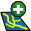
\includegraphics[width=0.7cm]{mActionAddNonDbLayer} 
Per caricare uno shapefile avviare QGIS e cliccare sul pulsante
\toolbtntwo{mActionAddNonDbLayer}{Aggiungi layer vettoriale}
\index{shapefile!caricamento} o semplicemente digitare \keystroke{V}. Lo stesso
strumento può essere usato per caricare qualunque dei formati supportati dalla
libreria OGR.

Cliccando sullo strumento si apre una finestra di dialogo standard (si veda la
Figura \ref{fig:openshapefile}) che consente di cercare nel filesystem lo
shapefile o qualunque altro dato vettoriale si intenda caricare. 
La casella di selezione \selectstring{Files of type}{\ldots} consente di
preselezionare alcuni formati supportati da OGR.

Se lo si desidera, può essere inoltre selezionata la codifica (encoding) da utilizzare per le
porzioni testuali della tabella dello shapefile.

\begin{figure}[ht]
   \begin{center}
   \caption{Finestra di dialogo Apri un layer vettoriale supportato da OGR \nixcaption}\label{fig:openshapefile}\smallskip
   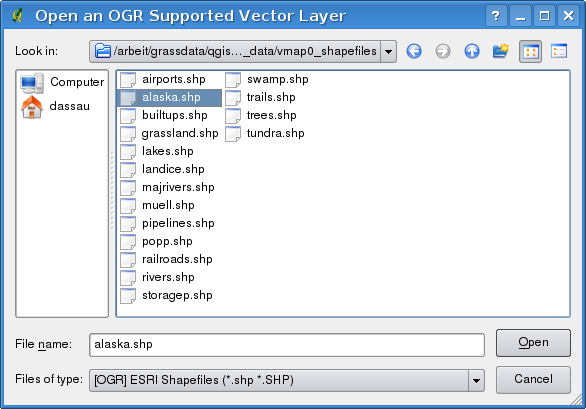
\includegraphics[clip=true, width=14cm]{shapefileopendialog}
\end{center} 
\end{figure}

Selezionando uno shapefile dalla lista e cliccando su \button{Open} esso viene
caricato in QGIS. La figura \ref{fig:loadedshapefile} mostra come appare
l'interfaccia di QGIS dopo aver caricato il file \filename{alaska.shp}.

\begin{figure}[ht]
   \begin{center}
   \caption{QGIS con lo shapefile Alaska caricato \nixcaption}\label{fig:loadedshapefile}\smallskip
   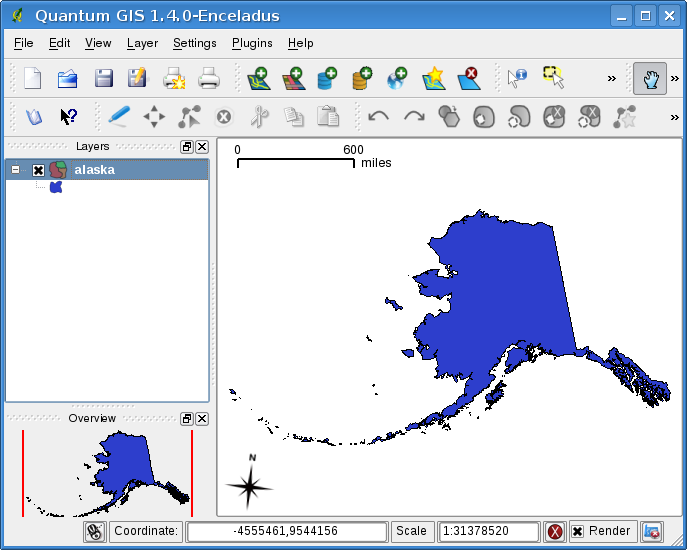
\includegraphics[clip=true, width=16cm]{shapefileloaded}
\end{center} 
\end{figure}

\begin{Tip}\caption{\textsc{Colori del layer}}
\qgistip{Quando un layer viene aggiunto alla mappa, gli viene assegnato un
colore a caso. Aggiungendo più layer in una sola volta, ad ognuno di essi
viene assegnato un colore differente. }
\end{Tip}

Una volta caricato, si può usare lo zoom nella mappa usando gli strumenti di navigazione.
Per cambiare la rappresentazione di un layer, aprire la finestra
\dialog{Proprietà} facendo doppio click sul nome del layer e quindi sulla
scheda Simbologia o cliccando con il
tasto destro sul nome del layer nella legenda e scegliendo
\dropmenuopt{Proprietà} dal menu contestuale. Si veda la Sezione
\ref{sec:symbology} per ulteriori informazioni su come settare la simbologia
dei layer vettoriali.

\subsubsection{Ottimizzare le prestazioni}

Per migliorare le prestazioni di disegno di uno shapefile, può essere creato
un indice spaziale. Un \index{indice spaziale!shapefile} indice spaziale
migliorerà la velocità di disegno quando si usano le funzioni di zoom e di
spostamento. Gli indici spaziali usati da QGIS hanno estensione \filename{.qix}.

Per creare un indice, seguire queste indicazioni:

\begin{itemize}
\item Caricare uno shapefile.
\item Aprire la finestra di dialogo \dialog{Proprietà} facendo doppio click
sul nome dello shapefile nella legenda o cliccando su di esso con il tasto
destro e scegliendo la voce \dropmenuopt{Proprietà} dal menu contestuale.
\item Nella scheda \tab{Generale} cliccare sul pulsante \button{Crea indice
spaziale}.
\end{itemize}

\subsubsection{Caricare un layer MapInfo}
\index{layer vettoriali!MapInfo}

Per caricare un layer MapInfo, cliccare nella barra strumenti sul pulsante
\toolbtntwo{mActionAddNonDbLayer}{Aggiungi layer vettoriale} o digitare
\keystroke{V}, cambiare il filtro sul tipo di file nel menu a tendina a
\selectstring{Files of Type}{[OGR] MapInfo (*.mif *.tab *.MIF *.TAB)} e
selezionare il layer che si intende caricare.

\subsubsection{Caricare una copertura ArcInfo}
\index{layer vettoriali!copertura ArcInfo}

Per caricare una copertura ArcInfo si usa lo stesso metodo precedentemente visto
per shapefile e layer MapInfo. 
Cliccare nella barra strumenti sul pulsante
\toolbtntwo{mActionAddNonDbLayer}{Aggiungi layer vettoriale} o digitare
\keystroke{V}, scorrere il filesystem per individuare la cartella contenente
la copertura che si vuole caricare e selezionare uno dei seguenti file (se
presenti nella propria copertura):

\begin{itemize}
\item \filename{.lab} - per caricare un layer etichette (etichette di poligoni o di punti).
\item \filename{.cnt} - per caricare un layer contenente i centroidi dei poligoni 
\item \filename{.arc} - per caricare un layer arc (linee).
\item \filename{.pal} - per caricare un layer di poligoni.
\end{itemize}

\subsection{Layer PostGIS}
\index{layer vettoriali!PostGIS|see{PostGIS}}
\index{PostGIS!layer}
\label{label_postgis} 

I layer sono immagazzinati in un database PostgreSQL. I vantaggi
nell'uso di PostGIS stanno nelle capacità fornite di creazione dell'indice spaziale,
di filtraggio e di interrogazione. Usando PostGIS, le funzioni
vettoriali come la selezione e l'identificazione in QGIS lavorano con maggiore
precisione che con i layer OGR.

Per usare layer PostGIS bisogna:\index{PostgreSQL!caricamento layer}

\begin{itemize}
\item Creare una connessione in QGIS con il database PostgreSQL (se non è già
definita).\index{PostgreSQL!connessione}
\item Connettersi al database.
\item Selezionare i layer da aggiungere alla mappa.
\item Fornire eventualmente una query SQL di tipo \usertext{where} per
definire quali elementi del layer caricare.
\item Caricare il layer.
\end{itemize}

\subsubsection{Creare una connessione}\index{PostgreSQL!connessione}\label{sec:postgis_stored}

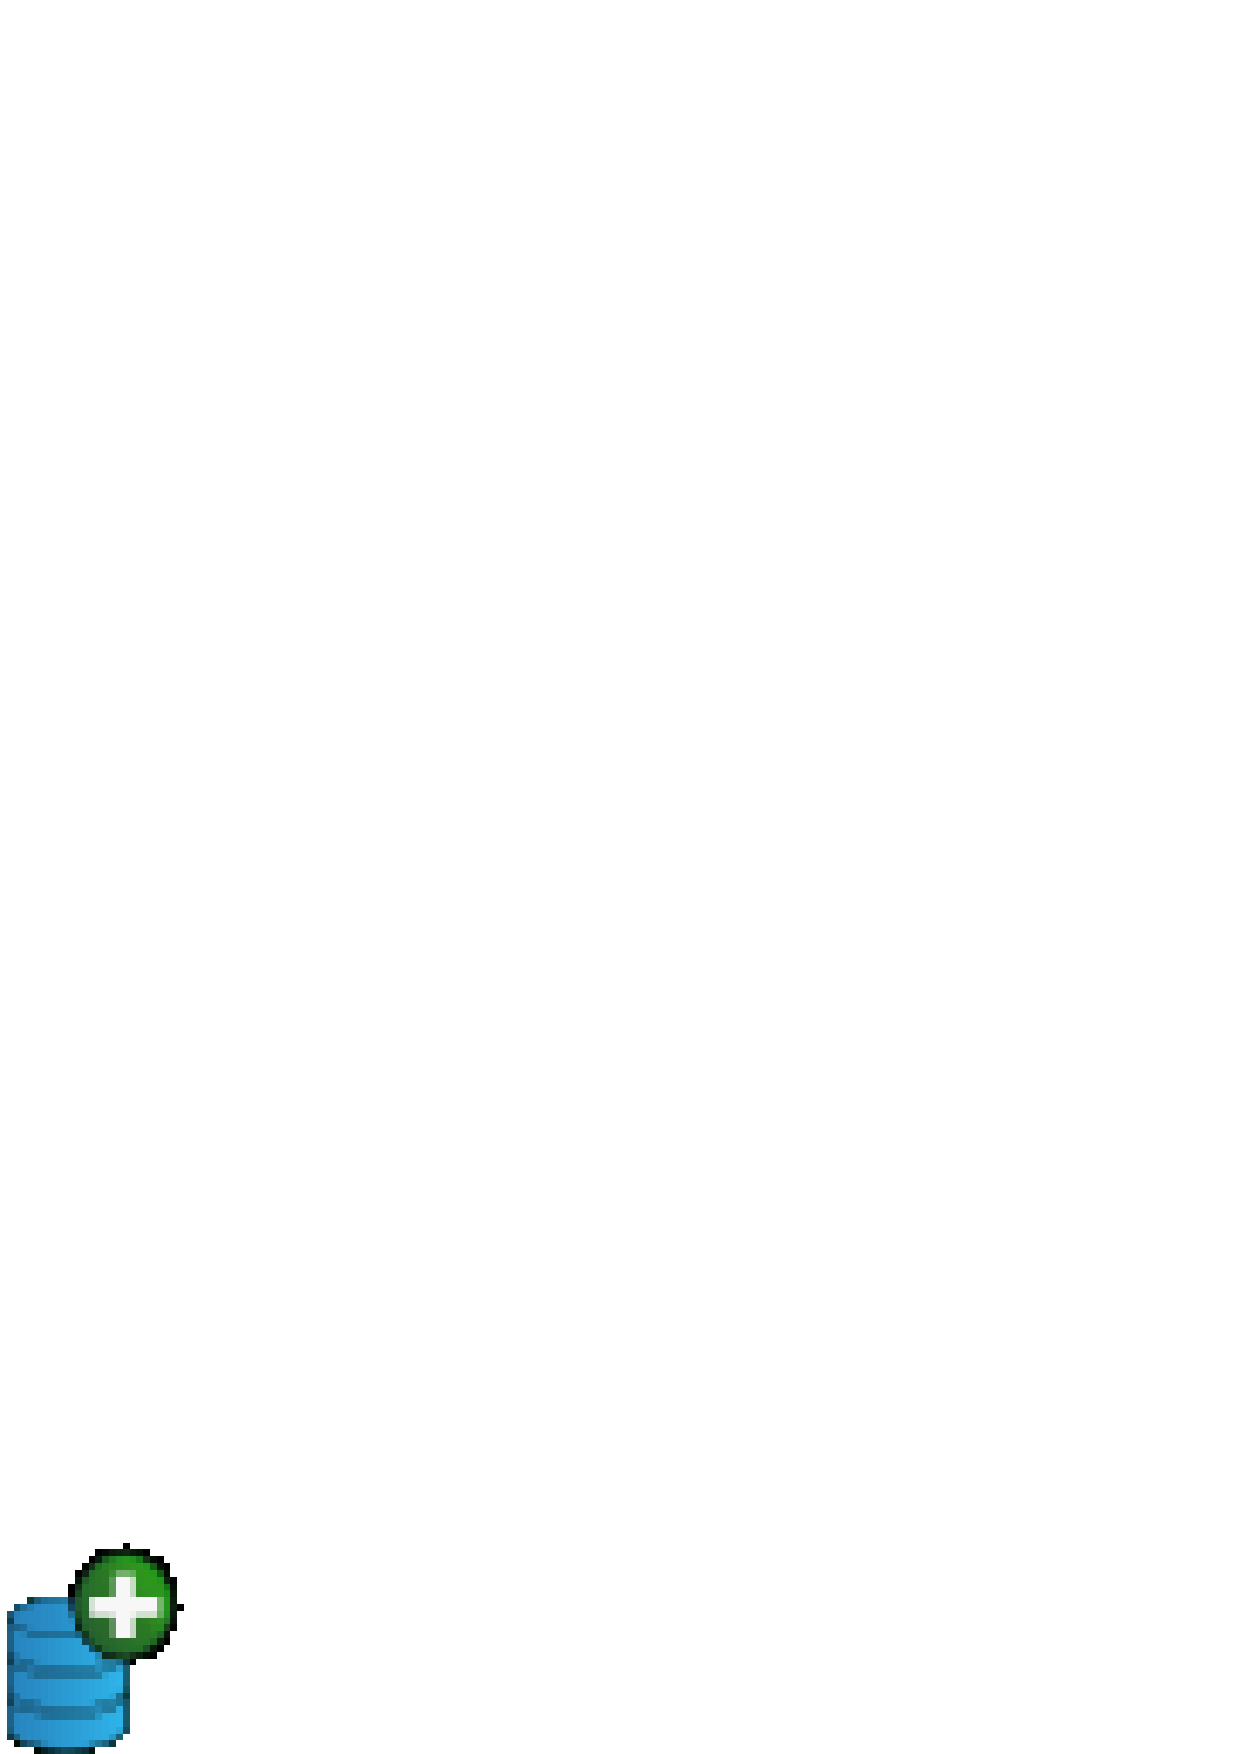
\includegraphics[width=0.7cm]{mActionAddLayer} La prima volta in cui viene
usata una fonte dati PostGIS, bisogna creare una connessione al database
PostgreSQL che contiene i dati. Cliccare nella barra strumenti sul pulsante
\toolbtntwo{mActionAddLayer}{Aggiungi layer PostGIS}, oppure selezionare l'opzione
\dropmenuopttwo{mActionAddLayer}{Aggiungi layer PostGIS...} dal menu
\mainmenuopt{Layer} o digitare \keystroke{D}. 
Si aprirà  la finestra di dialogo \dialog{Aggiungi tabella(e) PostGIS}. Per
accedere al gestore della connessione \index{PostgreSQL!gestore della connessione}
, cliccare sul tasto \button{Nuovo} per far comparire la finestra di
dialogo \dialog{Creare una nuova connessione PostGIS}. I parametri richiesti
per la connessione sono mostrati nella tabella \ref{tab:postgis_connection_parms}.

\begin{table}[ht]\index{PostgreSQL!parametri di connessione}
\centering
\caption{Parametri di connessione al geodatabase PostGIS}\label{tab:postgis_connection_parms}\medskip
 \begin{tabular}{|l|p{5in}|}
\hline Name & Nome della connessione. Può essere uguale a quello del \textsl{Database}.
\\
\hline Host \index{PostgreSQL!host}
& Nome del server che ospita il database. Deve essere un host con indirizzo
raggiungibile, lo stesso che potrebbe essere usato per aprire una connessione
telnet o per fare il ping all'host. Se il database è sullo stesso computer sul quale
è installato QGIS, inserire semplicemente "localhost". \\
\hline Database \index{PostgreSQL!database} & Nome del database.  \\
\hline Porta \index{PostgreSQL!porta}& Numero della porta sulla quale il
database PostgreSQL è in ascoloto. La porta di default è 5432.\\
\hline Username \index{PostgreSQL!nome utente}& Nome dell'utente che accede al
database. \\
\hline Password \index{PostgreSQL!password}& Password usata
dall'\textsl{Username} per collegarsi al database.\\
\hline
\end{tabular}
\end{table}

Come opzione, possono essere attivate le seguenti caselle di controllo:

\begin{itemize}
\item \checkbox{Salva password}
\item \checkbox{Cercare solamente nella tabella geometry\_columns}
\item \checkbox{Cerca solamente nello schema "public"}
\end{itemize}

Quando tutti i parametri sono impostati, la connessione può essere testata
cliccando sul pulsante \button{Prova connessione} \index{PostgreSQL!connessione!prova}.

\begin{Tip}\caption{\textsc{Definizione e sicurezza delle impostazioni utente in QGIS}}\index{impostazioni}\index{sicurezza}
\qgistip{Le impostazioni personalizzate di QGIS sono salvate in modo diverso
in base al sistema operativo. \nix, le impostazioni sono salvate nella
cartella home dell'utente nel file \filename{.qt/qgisrc}. \win, le
impostazioni sono salvate nel registro di sistema. Secondo il sistema
operativo, il salvataggio delle password in QGIS può essere più o meno a
rischio.
}
\end{Tip}

\subsubsection{Caricare un layer PostGIS}\index{PostgreSQL!caricamento layer}

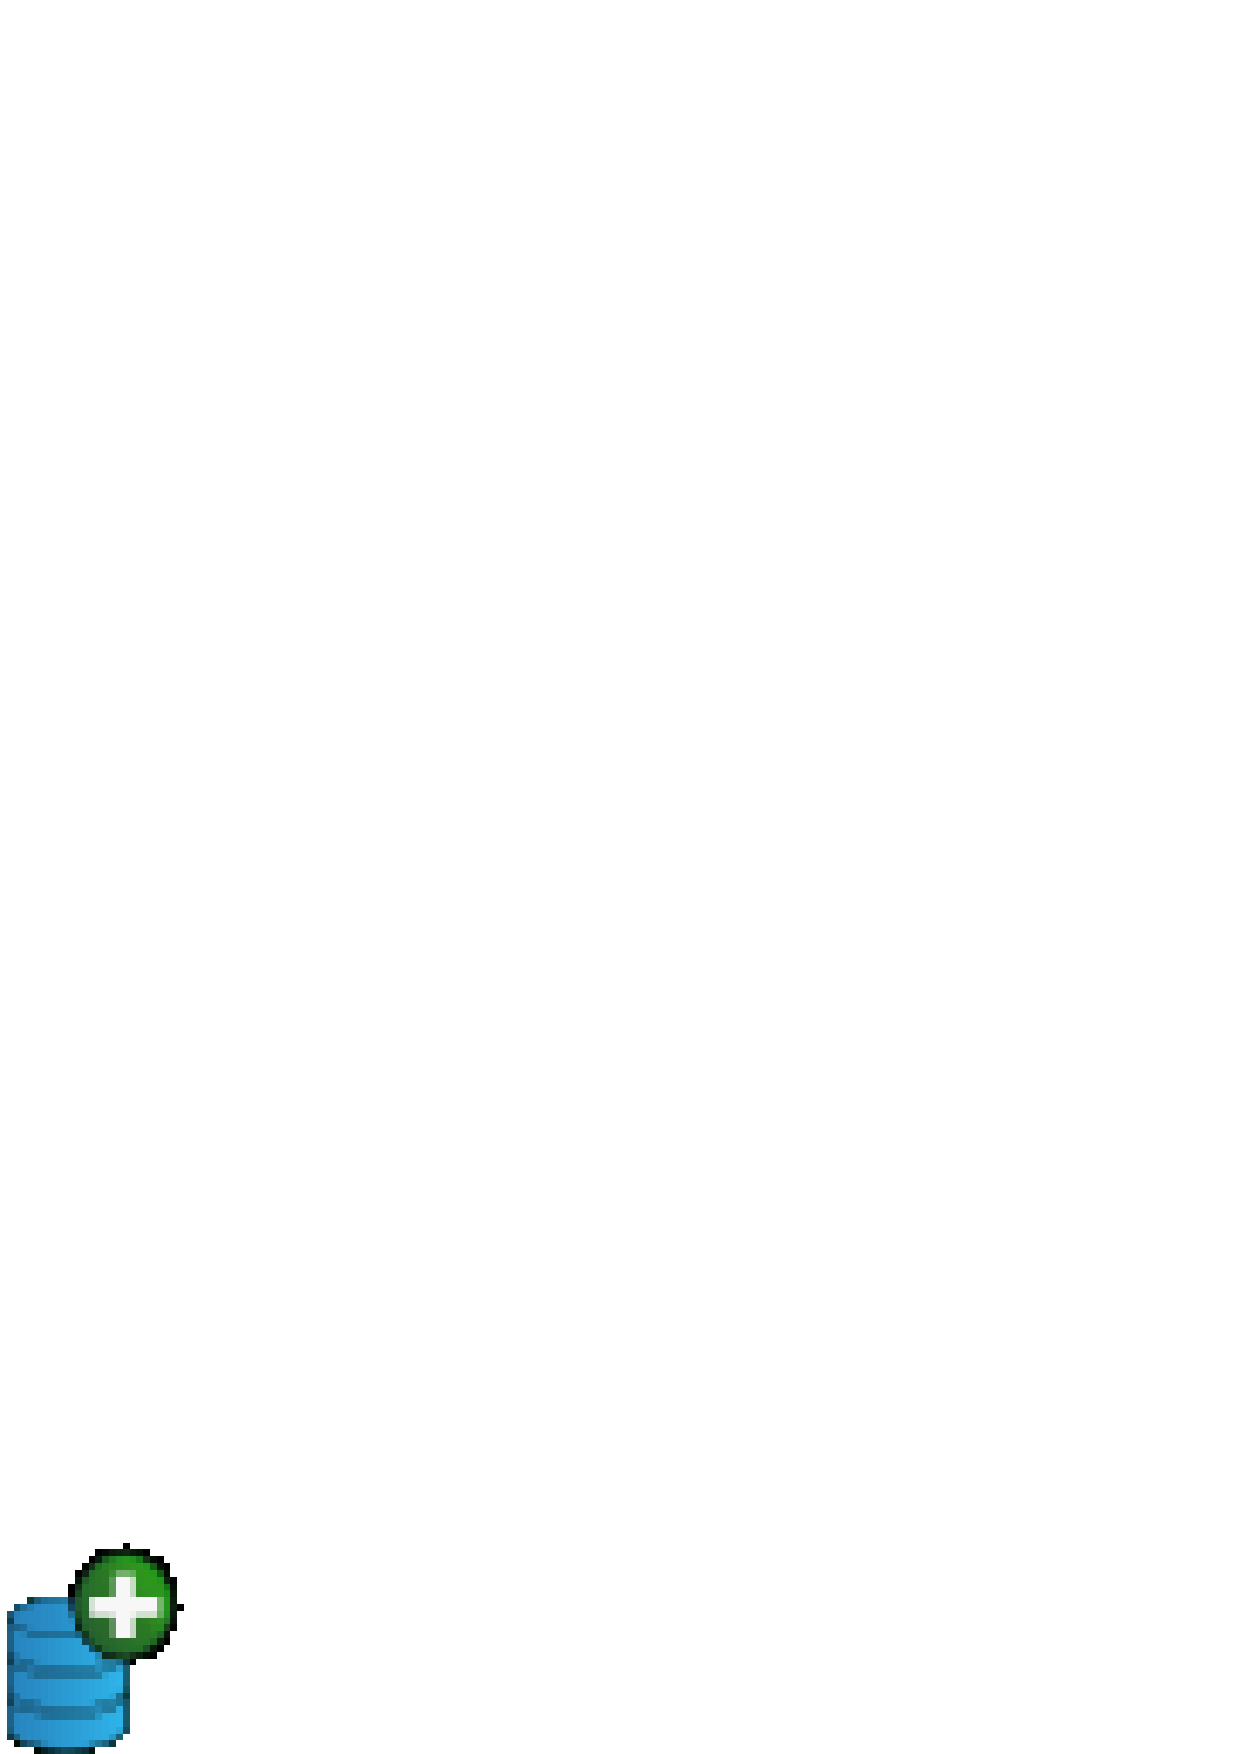
\includegraphics[width=0.7cm]{mActionAddLayer} Una volta definite una o più
connessioni, possono essere caricati layer dal database PostgreSQL.
Ovviamente questo richiede avere dati in PostgreSQL. Si veda la Sezione
\ref{sec:loading_postgis_data} per informazioni sul come importare dati nel
database. 

Per caricare layer da PostGIS, seguire i seguenti passaggi:

\begin{itemize}
\item Se la finestra di dialogo \dialog{Aggiungi tabella(e) PostGIS} non è già
aperta, cliccare nella barra strumenti sul pulsante
\toolbtntwo{mActionAddLayer}{Aggiungi layer PostGIS}.
\item Scegliere la connessione dal menu a tendina e cliccare su \button{Connetti}.
\item Individuare il layer che si vuole aggiungere nella lista fra quelli disponibili.
\item Selezionarlo cliccando sul nome. È possibile selezionare più layer
tenendo premuto il tasto \keystroke{shift} mentre si seleziona. Si veda la
Sezione \ref{sec:query_builder} per informazioni su come usare il costruttore
di query PostgreSQL per definire una selezione al momento del caricamento.
\item Cliccare sul tasto \button{Aggiungere} per aggiungere il livello alla mappa.
\end{itemize}

\begin{Tip}\caption{\textsc{layer PostGIS}}
\qgistip{Di solito un layer PostGIS è definito da un record nella tabella
geometry\_columns. Dalla versione \OLD % should be 0.9.0 
in avanti, QGIS può caricare layer che non hanno tale record nella tabella
geometry\_columns. Ciò vale sia per le tabelle che per le viste. La
definizione si una vista spaziale fornisce un mezzo molto potente per
visualizzare i dati. Fare riferimento al manuale PostgreSQL per informazioni
su come creare le viste.}
\end{Tip}

\subsubsection{Alcuni dettagli sui layer PostgreSQL}\label{sec:postgis_details}
\index{PostgreSQL!dettagli layer}

Questa sezione contiene alcuni dettagli su come QGIS accede ai layer
PostgreSQL. La maggior parte delle volte QGIS dovrebbe semplicemente fornire
una lista di tabelle del database che possono essere caricate, e caricarle su
richiesta. Tuttavia, se avete difficoltà a caricare una tabella di PostgreSQL
in QGIS, le informazioni qui sotto possono aiutare a capire tutti i messaggi di QGIS ed a
dare un'indicazione su come cambiare la definizione di tabella o di vista di PostgreSQL per permettere
a QGIS di caricarla.

QGIS richiede che i layer di PostgreSQL contengano una colonna che possa essere usata come
chiave unica per il layer. Per le tabelle questo significa che esse devono
contenere una chiave primaria o presentino una colonna con un vincolo unico su
essa. Se una tabella manca di questi
elementi, verrà usata la colonna oid. QGIS richiede inoltre che questa colonna sia di
tipo int4 (un numero intero del formato 4 byte). Le prestazioni saranno migliorate se la colonna è
indicizzata (notare che le chiavi primarie sono automaticamente indicizzate in PostgreSQL).

Se il layer di PostgreSQL è una vista, esistono gli stessi requisiti, ma le
viste non hanno chiavi primarie o colonne con i vincoli unici su di loro. In
questo caso QGIS proverà a trovare una colonna nella vista che provenga da una
colonna della tabella appropriata. Se non ne viene trovata alcuna, QGIS non
caricherà il layer. Se questo accade, la soluzione è di alterare la vista in
modo che includa una colonna adatta (un tipo di int4 e una chiave primaria o un vincolo unico, spostato e preferibilmente indicizzato).

\subsubsection{Importazione di dati in PostgreSQL}\label{sec:loading_postgis_data}
\index{PostGIS!SPIT!importazione dati}

\minisec{shp2pgsql}
I dati possono essere importati in PostgreSQL in diverse maniere. PostGIS
include un programma di utilità chiamato \filename{shp2pgsql} che può essere
usato per importare shapefile in un database PostGIS. Per esempio, per
importare lo shapefile chiamato \filename{lakes.shp}
nel database PostgreSQL chiamato \usertext{gis\_data}, usare il comando
seguente:

\begin{verbatim} 
  shp2pgsql -s 2964 lakes.shp lakes_new | psql gis_data
\end{verbatim}

Questo comando crea un nuovo layer chiamato \usertext{lakes\_new} nel database
{gis\_data}. Il nuovo layer avrà uno spatial reference identifier (SRID) di
2964. Si veda la Sezione \ref{label_projections} per ulteriori informazioni
sui sistemi di spatial reference systems e le proiezioni.
\begin{Tip}
\caption{\textsc{Esportare dati da PostGIS}\index{PostGIS!esportazione}}
\qgistip{Come è presente lo strumento per l'importazione \filename{shp2pgsql}
c'è anche lo strumento per l'esportazione di dati PostGIS come shapefile:
\filename{pgsql2shp}. Esso è incluso nella versione di PostGIS installata.} 
\end{Tip}

\minisec{SPIT Plugin}

\includegraphics[width=0.7cm]{spiticon} QGIS include un plugin denominato SPIT (Shapefile to PostGIS Import Tool)\index{PostGIS!SPIT}.
SPIT può essere usato per caricare più shapefile in una volta sola e
include il supporto per gli schemi. Per usare SPIT, aprire il QGIS Plugin Manager
dal menu \mainmenuopt{Plugins}, selezionare la casella di controllo vicina a
\checkbox{SPIT} e cliccate su \button{OK}. L'icona di SPIT verrà aggiunta alla
barra degli strumenti plugin\index{PostGIS!SPIT!caricamento}. 

Per importare uno shapefile, cliccare sull'icona
\toolbtntwo{spiticon}
nella barra degli strumenti per aprire la finestra di
dialogo \dialog{SPIT}.
Selezionare il database PostGIS al quale si desidera connettersi
e cliccare su \button{Connetti}.
Ora è possibile aggiungere uno o più file alla coda
cliccando su \button{Aggiungi}. Per processare i file selezionati, cliccare
su \button{OK}. L'avanzamento dell'importazione ed eventuali
errori/avvertimenti saranno mostrati mentre ciascuno shapefile viene
elaborato.
\begin{Tip}\caption{\textsc{Importare shapefile contenenti parole riservate in PostgreSQL}}\index{PostGIS!SPIT!parole riservate}
\qgistip{Se alla coda d'importazione uno shapefile contiene campi con parole riservate per il
database PostgreSQL, comparirà una finestra di dialogo
che darà informazioni sullo stato di ogni campo. È necessario editare i nomi
dei campi contenenti tali parole (ed è possibile eventualmente editare anche
il nome degli altri campi) \index{PostGIS!SPIT!editare il nome dei campi}
prima dell'importazione, altrimenti il processo di importazione non
andrà a buon fine.}
\end{Tip} 

\minisec{ogr2ogr}
Oltre a \filename{shp2pgsql} e \filename{SPIT} c'è un altro strumento per
inserire geodati in PostGIS: \filename{ogr2ogr}. Esso fa parte della versione
di GDAL installata.
Per importare uno shapefile in PostGIS con \filename{ogr2ogr}, digitare questo
comando:
\begin{verbatim}
  ogr2ogr -f "PostgreSQL" PG:"dbname=postgis host=myhost.de user=postgres \
  password=topsecret" alaska.shp
\end{verbatim}

L'espressione importerà lo shapefile \filename{alaska.shp} nel database PostGIS
\usertext{postgis}
usando l'utente \usertext{postgres} e la password \usertext{topsecret} sull'host
\server{myhost.de}.

Notare che OGR deve essere compilato con il supporto a PostgreSQL per poter
effettuare tale operazione.
La presenza del supporto a PostgreSQL-PostGIS può essere verificate digitando
da riga di comando:
\begin{verbatim}
ogrinfo --formats | grep -i post
\end{verbatim}

Se si volesse usare il comando interno di PostgreSQL \filename{COPY} al posto
del metodo predefinito \filename{INSERT INTO} bisogna settare le variabili
d'ambiente come segue (su piattaforme \nix e \osx):
\begin{verbatim}
  export PG_USE_COPY=YES
\end{verbatim}

\filename{ogr2ogr} non crea indici spaziali come \filename{shp2pgsl}. Bisogna
crearli manualmente usando il comando SQL \filename{CREATE INDEX} dopo
l'importazione come passaggio aggiuntivo (come descritto nella prossima
sezione \ref{label_improve}).

\subsubsection{Migliorare le prestazioni} \label{label_improve}

Richiamare dati geografici da un database PostgreSQL può richiedere molto
tempo, specialmente se il server dei dati si trova in rete. È possibile
migliorare le prestazioni di resa a video di layer PostgreSQL assicurandosi
di creare un \index{PostGIS!indice spaziale} indice spaziale su ogni layer nel
database. PostGIS supporta la creazione di un \index{PostGIS!indice
spaziale!GiST} indice GiST
(indice dell'albero generalizzato di ricerca, Generalized Search Tree) per
velocizzare le ricerche spaziali di dati.

La sintassi per la creazione di un indice GiST è:
\footnote{le informazioni sull'indice GiST
sono tratte dalla documentazione PostGIS disponibile su \url{http://postgis.refractions.net}}

\begin{verbatim}
    CREATE INDEX [indexname] ON [tablename] 
      USING GIST ( [geometryfield] GIST_GEOMETRY_OPS );
\end{verbatim}

Si noti che per tabelle molto grandi, la creazione dell'indice può richiedere
parecchio tempo. Non appena l'indice è stato creato, bisognerebbe effettuare
una \usertext{VACUUM ANALYZE}. Si veda la documentazione di PostGIS
\cite{PostGISweb} per ulteriori informazioni.

Ciò che segue è un esempio di come creare un indice GiST:
\begin{verbatim}
gsherman@madison:~/current$ psql gis_data
Welcome to psql 8.3.0, the PostgreSQL interactive terminal.

Type:  \copyright for distribution terms
        \h for help with SQL commands
        \? for help with psql commands
        \g or terminate with semicolon to execute query
        \q to quit

gis_data=# CREATE INDEX sidx_alaska_lakes ON alaska_lakes
gis_data-# USING GIST (the_geom GIST_GEOMETRY_OPS);
CREATE INDEX
gis_data=# VACUUM ANALYZE alaska_lakes;
VACUUM
gis_data=# \q
gsherman@madison:~/current$
\end{verbatim}

\subsubsection{Layer vettoriali che attraversano 180$^\circ$ di longitudine}
\index{vector layers!crossing}

Many GIS packages don't wrap vector maps, with a geographic reference system
(lat/lon), crossing the \degrees{180} longitude line. As result, if
we open such map in QGIS, we will see two far, distinct locations, that
should show near each other. In Figure \ref{fig:vector_not_wrapping} the tiny
point on the far left of the map canvas (Chatham Islands), should be within
the grid, right of New Zealand main islands.

\begin{figure}[ht]
   \begin{center}
   \caption{Map in lat/lon crossing the \degrees{180} longitude line
   \nixcaption}
   \label{fig:vector_not_wrapping}\smallskip
   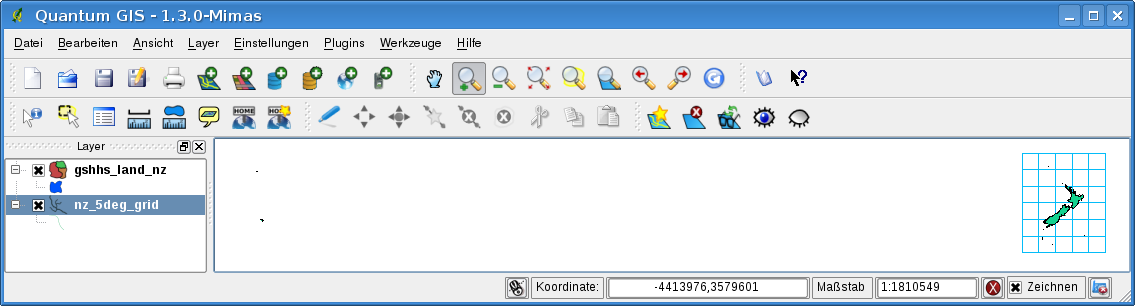
\includegraphics[clip=true, width=\textwidth]{vectorNotWrapping}
\end{center}
\end{figure}

A workaround is to transform the longitude values using PostGIS and the
\textbf{ST\textunderscore Shift\textunderscore Longitude}
\footnote{\url{http://postgis.refractions.net/documentation/manual-1.4/ST_Shift_Longitude.html}}
function. This function reads every point/vertex in every component of every
feature in a geometry, and if the longitude coordinate is < \degrees{0} adds
\degrees{360} to it. The result would be a \degrees{0} - \degrees{360} version of
the data to be plotted in a \degrees{180} centric map.

\begin{figure}[ht]
   \begin{center}
   \caption{Map crossing \degrees{180} longitude applying the ST\textunderscore Shift\textunderscore Longitude function \nixcaption}
\label{fig:vector_wrapping}\smallskip
   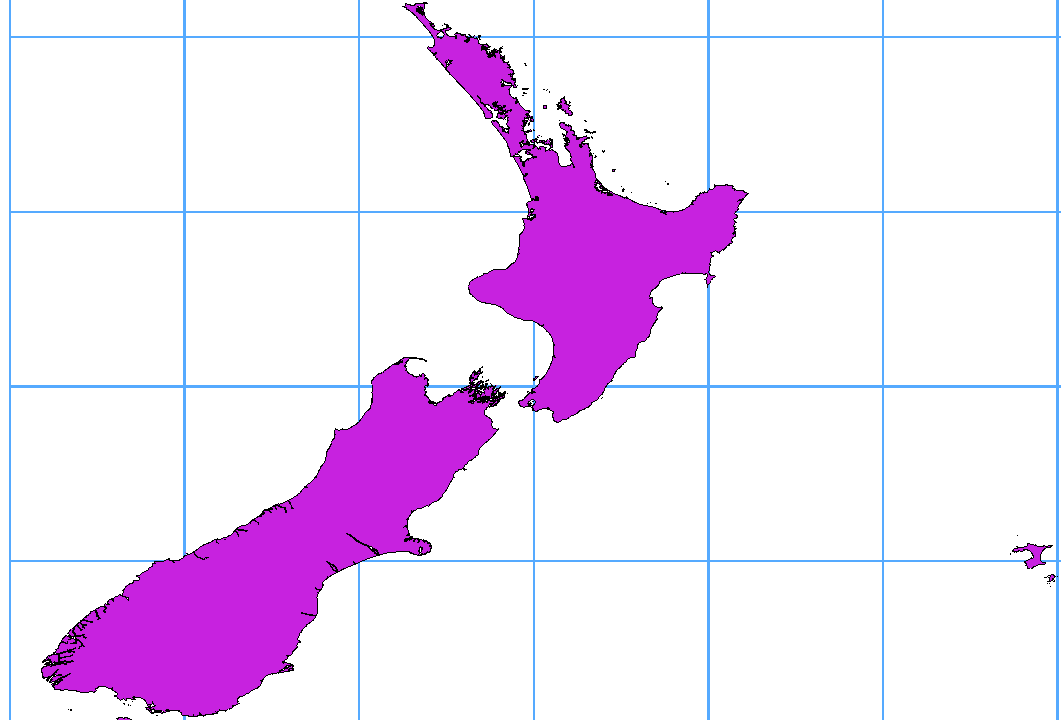
\includegraphics[clip=true, width=9cm]{vectorWrapping}
\end{center}
\end{figure}

\minisec{Utilizzo}

\begin{itemize}
\item Import data to PostGIS (\ref{sec:loading_postgis_data}) using for
example the PostGIS Manager plugin or the SPIT plugin
\item Use the PostGIS command line interface to issue the following command
(this is an example where "TABLE" is the actual name of your PostGIS table) \\ 
\texttt{gis\_data=\# update TABLE set the\_geom=ST\_shift\_longitude(the\_geom);} 
\item If everything went right you should receive a confirmation about the
number of features that were updated, then you'll be able to load the map and
see the difference (Figure \ref{fig:vector_wrapping})
\end{itemize}

\subsection{Layer SpatiaLite} 
\index{SpatiaLite layers!properties dialog}
\index{vector layers!SpatlaLIte|see{SpatiaLite}}
\index{SpatiaLite!layers}
\label{label_spatialite} 

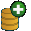
\includegraphics[width=0.7cm]{mActionAddSpatiaLiteLayer}
The first time you load data from a Spatialite database, begin by clicking on the 
\toolbtntwo{mActionAddSpatiaLiteLayer}{Add SpatiaLite Layer} toolbar button or by selecting the 
\dropmenuopttwo{mActionAddSpatiaLiteLayer}{Add SpatiaLite Layer...} 
option from the \mainmenuopt{Layer} menu or by typing \keystroke{L}. 
This will bring up a window, which will allow you to either connect to a Spatialite database already known to QGIS, which 
you can choose from the dropdown menu or to define a new connection to a new database. To define a new connection, 
click on \button{New} and use the file browser to point to your SpatiaLite database, 
which is a file with a \filename{.sqlite } extension.

\subsection{Proprietà dei layer vettoriali}\label{sec:vectorprops}
\index{layer vettoriali!finestra delle proprietà}

La finestra di dialogo \dialog{Proprietà del vettoriale} fornisce informazioni
sul layer, sulla sua rappresentazione grafica (simbologia) e opzioni per la
visualizzazione di etichette sugli elementi che lo compongono. Se il layer
vettoriale è stato caricato da un archivio dati PostgreSQL/PostGIS, è possbile
modificare anche l'espressione SQL che lo ha generato - sia a mano editando
l'espressione SQL nella scheda \tab{Generale} o richiamando la finestra di
dialogo \dialog{Costruttore di query} dalla scheda \tab{Generale}. 
Per accedere alla finestra di dialogo \dialog{Proprietà del vettoriale}, fare
doppio click sul layer nella legenda o click con il tasto destro  sul layer e
selezionare \dropmenuopt{Proprietà} dal menu contestuale.

\begin{figure}[H]
   \begin{center}
   \caption{Finestra delle proprietà di un vettoriale \nixcaption}\label{fig:vector_symbology}\smallskip
   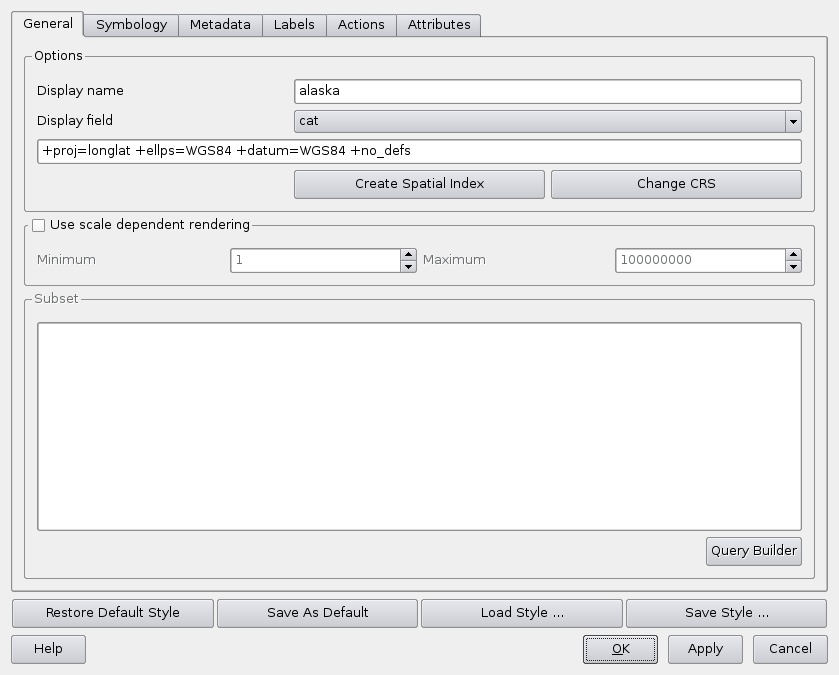
\includegraphics[clip=true, width=12cm]{vectorLayerSymbology} 
\end{center}  
\end{figure}

\subsubsection{Scheda Generale}\label{vectorgeneraltab}
La scheda \tab{Generale} è sostanzialmente simile a quella dei raster. Essa
consente di cambiare il nome del file mostrato, impostare la visualizzazione
in base alla scala, creare un indice spaziale (solo per i formati supportati
da OGR e per layer PostGIS) e vedere o cambiare la proiezione dello
specifico layer vettoriale.

Il pulsante \button{Creatore di query} consente di selezionare un sottoinsieme
di elementi nel layer - ma questo pulsante è attualmente disponibile
unicamente quando viene aperta la tabella attributi cliccando sul pulsante
\button{Avanzate ...}.

\subsubsection{Scheda simbologia}\label{sec:symbology}
\index{layer vettoriali!simbologia}

QGIS supporta diverse modalità di rappresentazione per controllare come gli
elementi dei layer vettoriali vengono mostrati. Attualmente sono disponibili le
seguenti modalità:

\begin{description} 
    \item[Simbolo singolo] - lo stesso stile è applicato a tutti gli elementi del vettore\index{layer vettoriali!stili!simbolo singolo}
    \item[Simbolo graduato] - lo stile applicato ai diversi elementi dipende
    dal valore di un campo particolare nella tabella associata.\index{layer vettoriali!stili!simbolo graduato}
    \item[Colore continuo] - gli elementi del layer sono mostrati con una
    gradazione di colori compresa entro due estremi specificati in base ai valori numerici di uno specifico campo.\index{layer vettoriali!stili!colore continuo}
    \item[Valore univoco] - gli oggetti sono classificati in base ai valori
    unici di uno specifico campo, ad ogni valore viene assegnata una
    simbologia differente.\index{layer vettoriali!stili!valore unico}
\end{description}

Per modificare la simbologia di un layer, fare semplicemente doppio click
sulla relativa voce di legenda per fare apparire la finestra di dialogo
\dialog{Proprietà del vettoriale}.\index{simbologia!modifica}

\begin{figure}[h]
\centering
\caption{Opzioni per la simbologia dei layer \nixcaption}
   \subfigure[Simbolo singolo] {\label{subfig:single_symbol}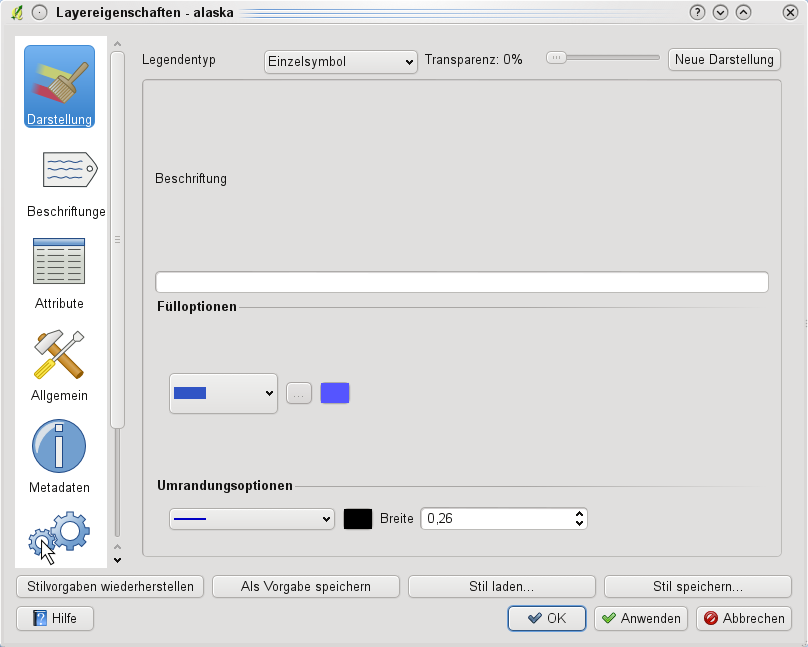
\includegraphics[clip=true, width=0.4\textwidth]{vectorClassifySingle}}\goodgap
   \subfigure[Simbolo graduato] {\label{subfig:graduated_symbol}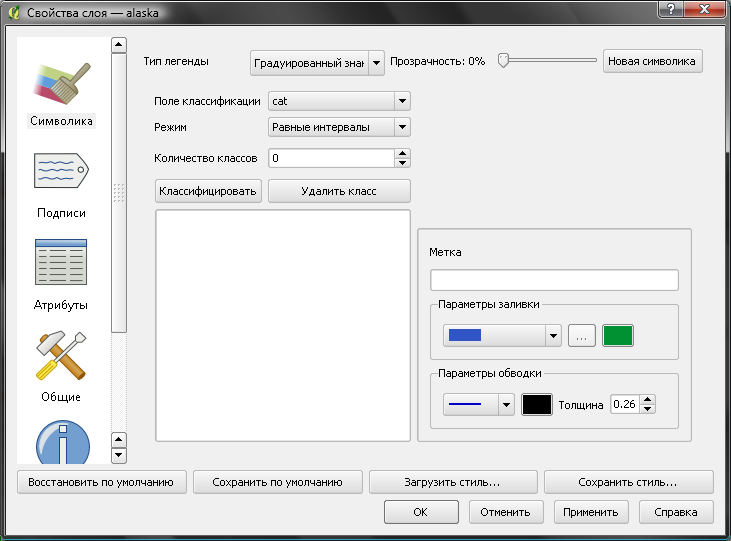
\includegraphics[clip=true, width=0.4\textwidth]{vectorClassifyGraduated}}\\
   \subfigure[Colore continuo] {\label{subfig:cont_color}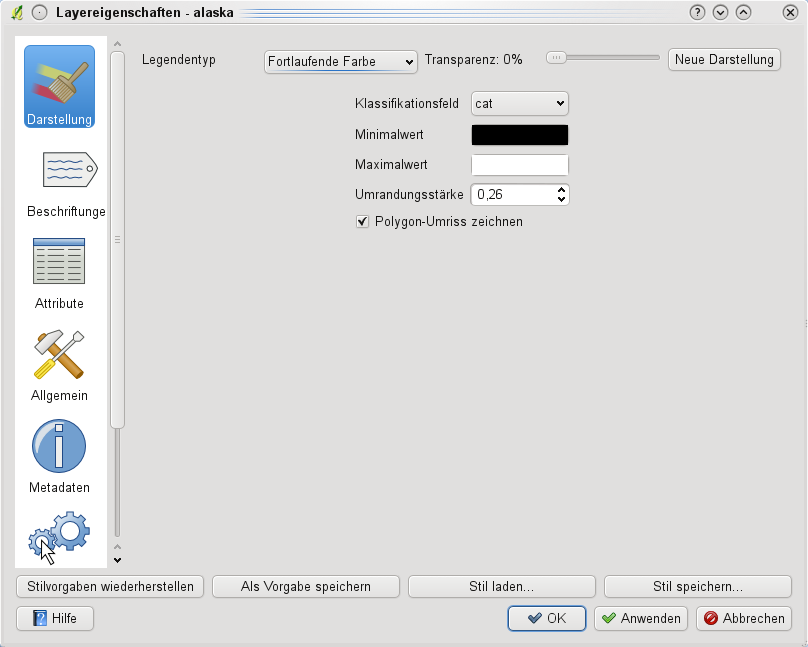
\includegraphics[clip=true, width=0.4\textwidth]{vectorClassifyContinous}}\goodgap
   \subfigure[Valore unico] {\label{subfig:unique_val}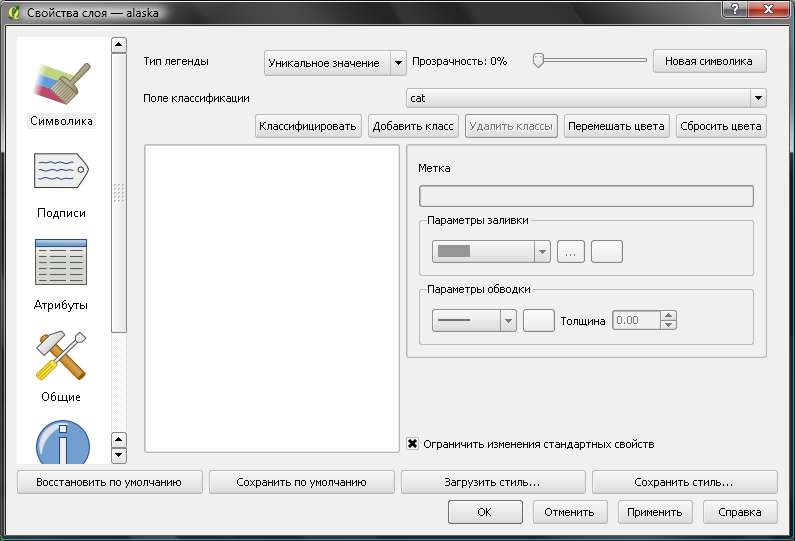
\includegraphics[clip=true, width=0.4\textwidth]{vectorClassifyUnique}}
\end{figure}

% FIXME: outdated
% Since \usertext{version v0.9} there is a function to use image files stored on 
% your computer as fill pattern for vector layers.

\minisec{Opzioni per lo stile} \label{sec:style_options} \index{layer vettoriali!stili}
In questa finestra di dialogo è possibile scegliere lo stile di
rappresentazione del layer vettoriale. Secondo l'opzione di visualizzazione
scelta tra quelle descritte precedentemente si ha la possibilità di
classificare anche gli elementi della mappa.

Le seguenti opzioni dovrebbero essere disponibili per pressoché tutte le
simbologie:
\begin{description}
 \item[Stile esterno] - tipo di tratteggio del contorno degli elementi. Si può
 anche impostare l'opzione "Nessuna penna" per escludere la rappresentazione
 del contorno.
 \item[Colore esterno] - colore del contorno degli elementi
 \item[Dimensione stile esterno] - larghezza della linea di contorno
 \item[Colore di riempimento] - colore di riempimento degli elementi.
 \item[Stile di riempimento] - stile per il riempimento. Oltre ai retini forniti è possibile scegliere \selectstring{Stile di riempimento}{? Texture} e cliccare su \browsebutton per selezionare un retino personalizzato. Attualmente sono supportati i formati \filename{*.jpeg, *.xpm, and *.png}.
\end{description}

Una volta impostato lo stile del layer esso può essere salvato in un fil
separato (con estensione \filename{*.qml}).
Per fare ciò, cliccare sul pulsante \button{Salva stile \ldots}. Ovviamente il
pulsante \button{Caricamento stile \ldots} carica un file di stile precedentemente
salvato.

Se si desidera usare sempre un particolare stile quando il layer viene
caricato, cliccare su \button{Salva come predefinito} per rendere predefinito
lo stile impostato. Inoltre, se si effettuano allo stile modifiche delle quali
non si è soddisfatti, cliccare su \button{Ripristina stile predefinito} per
ritornare allo stile predefinito precedentemente impostato.

\minisec{Applicare la trasparenza ad un vettore} \label{sec:vect_transparency} \index{layer
vettoriali!trasparenza}
QGIS \CURRENT fornisce la possibilità di settare la trasparenza per ogni layer
vettoriale. Ciò può essere fatto settando l'apposita barra
\slider{Trasparenza}{0}{20mm} nella scheda \tab{Symbologia} (si veda la fig. \ref{fig:vector_symbology}).
Ciò può essere molto utile per la visualizzazione di più layer vettoriali
sovrapposti.

\subsubsection{New Generation Symbology}

In QGIS \CURRENT a new symbology was integrated in parallel with the symbology 
described above. This new generation symbology provides a variety of improvements and 
new features and will replace the current symbology in one of the upcoming releases. 
To switch to the new symbolgy you currently have to click on the \button{new symbology} button in the \tab{General} tab of the \dialog{Layer Properties} dialog.  

\minisec{Understanding the new generation symbology}

There are three types of symbols: marker symbols (for points), line symbols and 
fill symbols (for polygons). Symbols can consist of one or more symbol layers. It 
is possible to define the color of a symbol and this color is then defined for all 
symbol layers. Some layers may have the color locked - for those the color can not 
be altered. This is useful when you define the color of a multilayer symbol. 
Similarly, it is possible to define the width for line symbols, as well as size and 
angle for marker symbols.

\minisec{Available symbol layer types} 

\begin{itemize}
\item \textbf{Simple marker}: Rendering with one of hardcoded markers.
\item \textbf{Simple line}: Usual rendering of a line (with specified 
width, color and pen style) 
\item \textbf{Simple fill}: Usual rendering of a polygon (with defined 
fill color, fill pattern and outline) 
\item \textbf{SVG marker}: Rendering with a SVG picture 
\item \textbf{Marker line}: A line rendered by repeating a marker symbol 
\end{itemize}

\minisec{Color ramps}

Color ramps are used to define a range of colors that can be used during 
the creation of renderers. The symbol's color will be set from the color ramp. 
There are two types of color ramps:
 
\begin{itemize}
\item \textbf{Gradient}: Linear gradient from one color to some other.
\item \textbf{random}: Randomly generated colors from a specified area of 
color space 
\end{itemize}

\minisec{Styles}

A style groups a set of various symbols and color ramps. You can define your 
prefered or frequently used symbols, and can use it  without having to recreate 
it everytime. Style items (symbols and color ramps) have always a name by which 
they can be queried from the style. There is one default style in QGIS (modifiable) 
and the user can add further styles.

\minisec{Renderers}

The renderer is responsible for drawing a feature together with the correct 
symbol. There are three types of renderers: single symbol, categorized (called 
unique color in the old symbology), and graduated. There is no continuous color 
renderer, because it is in fact only a special case of the graduated renderer. 
The categorized and graduated renderer can be created by specifying a symbol 
and a color ramp - they will set the colors for symbols appropriately. 

\subsubsection{Working with the New Generation Symbology}

First you have to enable the new generation symbology clicking on the 
\button{new symbology} button in the \tab{General} tab of the 
\dialog{Layer Properties} dialog. The new dialog allows to choose one of the 
three renderers: single symbol, categorized and graduated. Depending on the 
chosen renderer, the symbology tab provides different settings and options, that 
will be described in the following sections.

\minisec{Single Symbol Renderer}

The Single Symbol Renderer is used to render all features of the layer using a 
single user-defined symbol. The properties, that can be adjusted in the 
Symbology tab, depend partially on the type of the layer, but all types share 
the following structure. In the top left part of the tab, there is a preview of 
the current symbol to be rendered. In the bottom part of the tab, there is a 
list of symbols already defined for the current style, prepared to be used via 
selecting them from the list. The current symbol can be modified using the 
\button{Properties} button, which opens a \dialog{Symbol Properties} dialog, or 
the \button{Set Color} button, which opens an ordinary \dialog{Color} dialog.
After having done any needed changes, the symbol can be added to the list of 
current style symbols (using the \button{Add to style} button) and then easily 
be used in the future.
 
\begin{figure}[h]
\centering
\caption{New Single Symbolizing options \nixcaption}
   \subfigure[Single symbol point properties] {\label{subfig:singleNG1}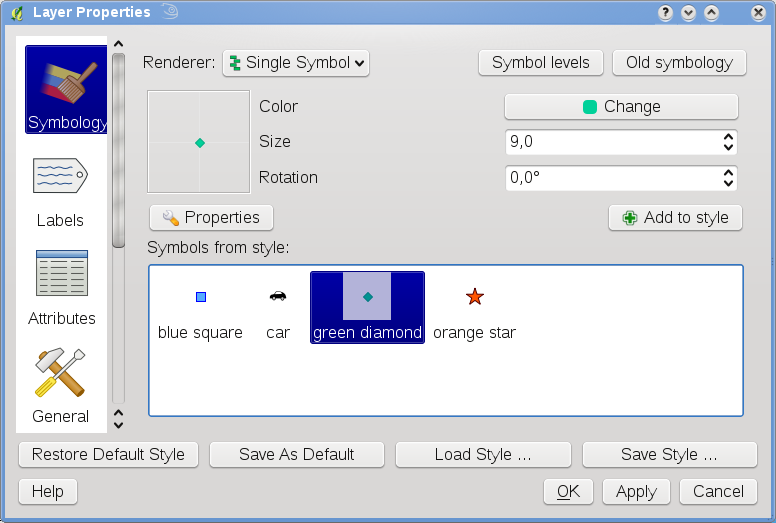
\includegraphics[clip=true, width=0.3\textwidth]{singlesymbol_ng_point}}\goodgap
   \subfigure[Single symbol line properties] {\label{subfig:singleNG2}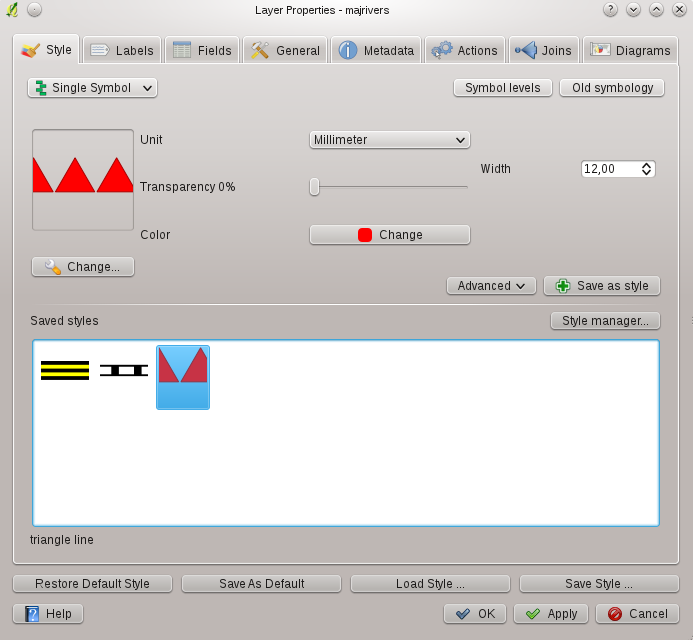
\includegraphics[clip=true, width=0.3\textwidth]{singlesymbol_ng_line}}\goodgap
   \subfigure[Single symbol area properties] {\label{subfig:singleNG3}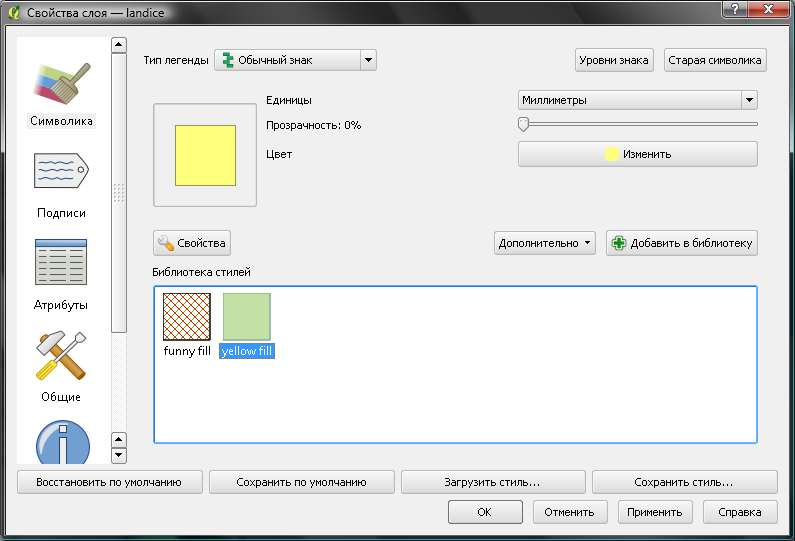
\includegraphics[clip=true, width=0.3\textwidth]{singlesymbol_ng_area}}
\end{figure}

\minisec{Categorized Renderer}

The Categorized Renderer is used to render all features from a layer, using a 
single user-defined symbol, which color reflects the value of a selected 
feature's attribute. The Symbology tab allows you to select:

\begin{itemize}
\item The attribute (using the Column listbox)
\item The symbol (using the Symbol Properties dialog)
\item The colors (using the Color Ramp listbox)  
\end{itemize}

For convenience, the list in the bottom part of the tab lists the values of 
all currently selected attributes together, including the symbols that will 
be rendered.

The example in figure \ref{fig:catsymNG} shows the category rendering dialog 
used for the rivers layer of the qgis sample dataset.

\begin{figure}[ht]
   \begin{center}
   \caption{New Categorized Symbolizing options \nixcaption}\label{fig:catsymNG}\smallskip
   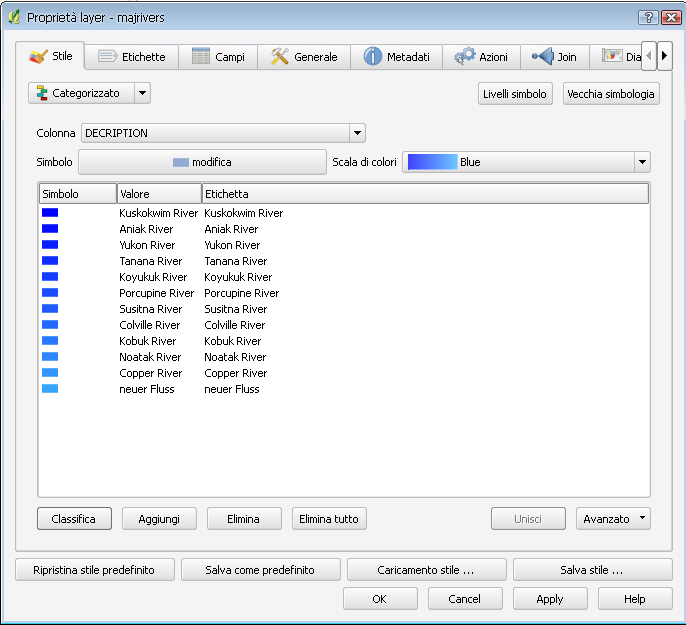
\includegraphics[clip=true, width=10cm]{categorysymbol_ng_line}
\end{center}
\end{figure}

\minisec{Graduated rendering}

The Graduated Renderer is used to render all the features from a layer, using 
a single user-defined symbol, whose color reflects the classification of a selected 
feature's attribute to a class.

Analogue to the categorized rendered, the symbology tab allows you to select:

\begin{itemize}
\item The attribute (using the Column listbox)
\item The symbol (using the Symbol Properties button)
\item The colors (using the Color Ramp list)
\end{itemize}

Additionally, you can specify the number of classes and also the mode how to 
classify features inside the classes (using the Mode list). The listbox in the 
bottom part of the symbology tab lists the classes together with their ranges, 
labels and symbols that will be rendered.

The example in figure \ref{fig:gradsymNG} shows the category rendering dialog 
for the rivers layer of the qgis sample dataset.

\begin{figure}[ht]
   \begin{center}
   \caption{New Graduated Symbolizing options \nixcaption}\label{fig:gradsymNG}\smallskip
   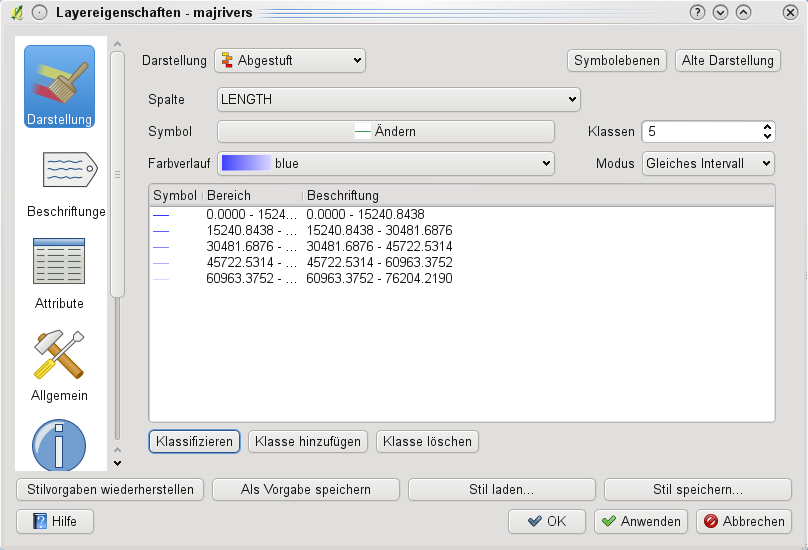
\includegraphics[clip=true, width=10cm]{graduatesymbol_ng_line}
\end{center}
\end{figure}

\minisec{Symbol Properties}

The symbol properties dialog allows the user to specify different properties of 
the symbol to be rendered. In the top left part of the dialog, you find a preview 
of the current symbol as it will be displayed in the map canvas. Below the preview 
is the list of symbol layers. To start the symbol properties dialog, click the 
\dropmenuopttwo{mActionOptions}{Properties} button in the \tab{General} tab of the
\dialog{Layer Properties} dialog. 

The control panels allow adding or removing layers, changing the position of layers, 
or locking layers for color changes. In the right part of the dialog, there are 
shown the settings applicable to the single symbol layer selected in the symbol 
layer list. The most important is the 'Symbol Layer Type' combo box, which allows 
you to choose the layer type. The available options are \filename{SimpleLine}, 
\filename{SvgMarker} and \filename{SimpleFill}. 

Depending on the chosen value, these settings are available in the right part 
of the dialog:

\begin{itemize}
\item \textbf{SimpleLine}: Color, Pen width, Pen style, Offset, Join style and Cap style; 
\item \textbf{SvgMarker}: Size, Angle, Offset X, Offset Y and SVG Image
\item \textbf{SimpleFill}: Color, Border color, Fill style. 
\end{itemize}

Example: A picture showing a line symbol composed from three simple lines with different pen widths. 
Example: Symbol properties for a point layer
Example: Symbol properties filling pattern for a polygon layer

\begin{figure}[h]
\centering
\caption{Defining symbol properties \nixcaption}
   \subfigure[Line composed from three simple lines] {\label{subfig:symprops1}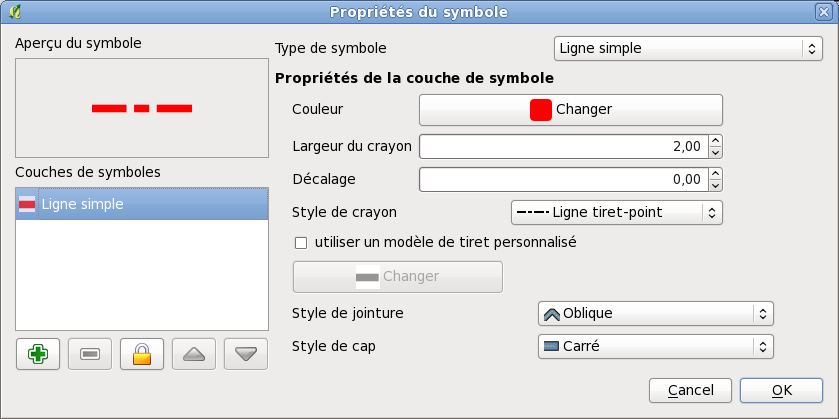
\includegraphics[clip=true, width=0.3\textwidth]{symbolproperties1}}\goodgap
   \subfigure[Symbol properties for point layer] {\label{subfig:symprops2}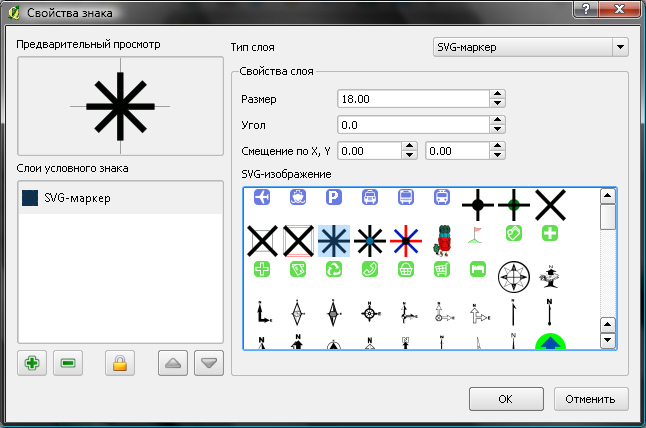
\includegraphics[clip=true, width=0.3\textwidth]{symbolproperties2}}\goodgap
   \subfigure[Filling pattern for a polygon] {\label{subfig:symprops3}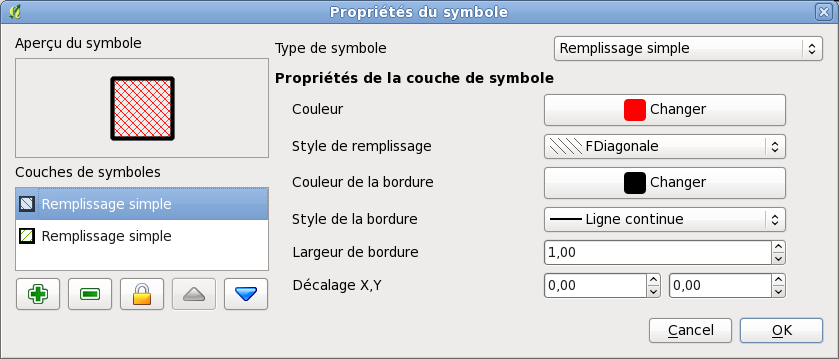
\includegraphics[clip=true, width=0.3\textwidth]{symbolproperties3}}
\end{figure}

\subsubsection{Style Manager to manage symbols and color ramps}

The Style Manger is a small helper application, that lists symbols and color 
ramps available in a style. It also allows you to add and/or remove items. To 
launch the Style Manager, click on \mainmenuopt{Settings} > \dropmenuopt{Style 
Manager} in the mai menu.

\begin{figure}[ht]
   \begin{center}
   \caption{Style Manager to manage symbols and color ramps \nixcaption}\label{fig:stylemanager}\smallskip
   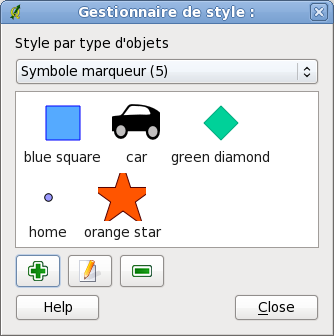
\includegraphics[clip=true, width=7cm]{stylemanager}
\end{center}
\end{figure}

\subsubsection{Scheda Etichette}

La scheda \tab{Etichette} consente di abilitare la visualizzazione delle
etichette associate agli elementi del layer e controlla una serie di
opzioni legate al posizionamento, allo stile e ad altre caratteristiche delle
etichette.

Come esempio apporremo le etichette allo shapefile lakes del
\filename{dataset\_esempio\_di\_qgis}:

\begin{enumerate}
\item Caricare lo shapefile \filename{alaska.shp} e il file GML \filename{lakes.gml} in QGIS.
\item Usare lo zoom su un'area a scelta contenente alcuni laghi.
\item Rendere attivo il layer \filename{lakes} cliccando su di esso nella
legenda.
\item Aprire la finestra di dialogo \dialog{Proprietà del vettoriale}.
\item Cliccare sulla scheda \tab{Etichette}.
\item Selezionare la casella di controllo \checkbox{Mostra etichette} per
abilitarne la visualizzaizone.
\item Scegliere il campo della tabella contenente le etichette da apporre. 
  In questo esempio si userà il \selectstring{Campo contenente etichetta}{NAMES}.
\item Inserire una etichetta di default per gli elementi del layer lakes che
non hanno nome. Questa etichetta verrà quindi usata ogni volta che QGIS dovrà
etichettare un lago al quale non corrisponda un valore nel campo \guilabel{NAMES}.
\item Cliccare su \button{Apply}.
\end{enumerate} 

Adesso sono visualizzate le etichette. Il loro aspetto non è probabilmente
gradevole, potrebbero essere troppo grandi e posizionate male in relazione al
simbolo dei laghi.

Cliccare allora su \button{Carattere} e \button{Colore}
per impostare il tipo di carattere e il colore. È possibile anche cambiare
l'angolo e la posizione delle etichette testuali.

Per modificare la posizione relativa del testo rispetto agli elementi:

\begin{enumerate} 
\item Cliccare sulla scheda \tab{Etichette}.
\item Cambiare la posizione selezionando una delle opzioni disponibili nel
gruppo \classname{Posizionamento}. Nel caso preso in esame, scegliere l'opzione
\radiobuttonon{Destra}.
\item la voce \classname{Unità della dimensione del carattere} consente di
selezionare tra \radiobuttonon{Punti} o \radiobuttonon{Unità mappa}.
\item Cliccare su \button{Apply} per visualizzare i cambiamenti senza chiudere
la finestra di dialogo.
\end{enumerate} 

Ora l'aspetto sarà migliore, ma le etichette appaiono ancora troppo vicine
all'indicatore della loro posizione. Per sistemare il problema è possibile
utilizzare l'opzione della voce \tab{Posizione}. Può qui essere impostato uno
scostamento nelle direzioni X e Y. Aggiungendo uno spostamento in X pari a 5
le etichette verrano scostate dall'indicatore della loro posizione e rese
più leggibili. Ovviamente più è grande l'indicatore o il carattere, maggiore
sarà lo scostamento da applicare.

Aggiungiamo infine un buffer sulle etichette cliccando sulla voce
\tab{buffer}. In questo modo verrà aggiunto uno sfondo attorno alle lettere
per farle risaltare maggiormente. Per mettere un buffer alle etichette dei
laghi procedere come di seguito:

\begin{enumerate}
\item Cliccare sulla voce \tab{Buffer}.
\item Abilitare la casella di controllo \checkbox{Buffer sulle etichette?}.
\item Scegliere una dimensione (spessore) del buffer.
\item Scegliere un colore per il buffer cliccando sul pulsante
\button{Colore}. È inoltre possibile assegnare una trasparenza in percentuale
al buffer.
\item Cliccare su \button{Apply} per vedere giudicare i cambiamenti.
\end{enumerate} 

Modificare eventualmente i cambiamenti fino a quando non si è soddisfatti del
risultato, cliccando su \button{Apply} dopo ogni modifica.

In genere un buffer di 1 punto fornisce risultati esteticamente gradevoli.
Si noti che è anche possibile specificare la dimensione del buffer in unità
della mappa se ciò rende più agevole l'impostazione.

Le rimanenti voci della scheda \tab{Etichette} consentono di controllare
l'aspetto delle etichette usando, se adeguatamente preparati, gli attributi
del layer. Le voci che iniziano con \tab{Definizione} consentono di settare
tutti i parametri delle etichette facendo riferimento a campi della tabella
del layer.

Si noti che la scheda \tab{Etichette} fornisce una \classname{Anteprima}
nella quale viene mostrata l'etichetta predefinita.

\subsubsection{Attributes Tab}\index{Attributes}\label{label_attributes}

Within the \tab{Attributes} tab the attributes of the selected dataset can be
manipulated. The buttons \toolbtntwo{mActionNewAttribute}{New Column} and
\toolbtntwo{mActionDeleteAttribute}{Delete Column} can be
used, when the dataset is \toolbtntwo{mActionToggleEditing}{editing mode}.
At the moment only columns from PostGIS layers can be removed and added. The
OGR library supports to add new columns, but not to remove them, if you have
a GDAL version >= 1.6 installed.

\minisec{edit widget}

\begin{figure}[H]
   \begin{center}
   \caption{Dialog to select an edit widget for an attribute column
\nixcaption}\label{fig:editwidget}\smallskip
   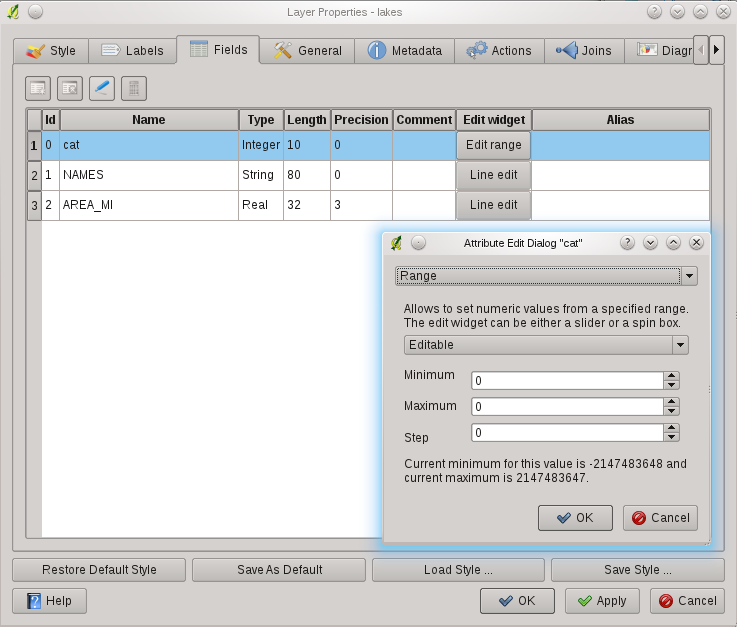
\includegraphics[clip=true, width=14cm]{editwidgetsdialog}
\end{center}
\end{figure}

Within the \tab{Attributes} tab you also find an \texttt{edit widget} column.
This column can be used to define values or a range of values that are
allowed
to be added to the specific attribute table column. If you click on the
\button{edit widget} button, a dialog opens, where you can define different
widgets. These widgets are:

\begin{itemize}
\item Line edit: an edit field which allows to enter simple text (or restrict
to
numbers for numeric attributes).
\item Classification: Displays a combo box with the values used for
classification, if you have chosen 'unique value' as legend type in the
symbology tab of the properties dialog.
\item Range: Allows to set numeric values from a specific range. The edit
widget can be either a slider or a spin box.
\item Unique value: The user can select one of the values already used in the
attribute table. If editable is activated, a line edit is shown with
autocompletion support, otherwise a combo box is used.
\item File name: Simplifies the selection by adding a file chooser dialog.
\item Value map: a combo box with predefined items. The value is stored in
the attribute, the description is shown in the comboo box. You can define
values manually or load them from a layer or a csv file.
\item Enumeration: Opens a combo box with values that can be used within the
columns type. This is currently only supported by the postgres provider.
\item Immutable: The immutable attribute column is read-only. The user is not
able to modify the content.
\end{itemize}

\subsubsection{General Tab}\label{vectorgeneraltab}

The \tab{General} tab is essentially like that of the raster dialog. It
allows you to change the display name, set scale dependent rendering options,
create a spatial index of the vector file (only for OGR supported formats and
PostGIS) and view or change the projection of the specific vetor layer.

The \button{Query Builder} button allows you to create a subset of the
features in the layer - but this button currently only is available when you
open the attribute table and select the \button{...} button next to Advanced
search.

\subsubsection{Metadata Tab}\index{Metadata}

The \tab{Metadata} tab contains general information about the layer,
including specifics about the type and location, number of features, feature
type, and the editing capabilities. The \guiheading{Extents} section,
providing
layer extent information, and the \guiheading{Layer Spatial Reference System}
section, providing information about the CRS of the layer. This is a quick
way to get information about the layer, but is not yet editable.

\subsubsection{Scheda Azioni}\index{azioni}\label{label_actions}

QGIS offre la possibilità di effettuare azioni sulla base degli
attributi associati ai singoli elementi del layer vettoriale.
Questo permette di effettuare un elevato numero di azioni, per esempio,
lanciare un programma con argomenti costruiti tramite gli attributi
delle geometrie o passando i parametri ad uno strumento di web reporting.

Definire delle azioni è utile quando si voglia lanciare un'applicazione
esterna o la visualizzazione di una pagina web sulla base di uno o più valori
associati al layer vettoriale. Ad esempio si può lanciare una ricerca web
basata sul valore di un attributo. Questo concetto è spiegato nel seguente
paragrafo.

\minisec{Definire le azioni}\index{azioni!definizione}

Le azioni legate agli attributi sono definite dalla finestra di dialogo
\dialog{Proprietà del vettoriale}. Per impostare un'azione, aprire la finestra
di dialogo \dialog{Proprietà del vettoriale} e cliccare sulla scheda
\tab{Azioni}. Fornire una descrizione per l'azione nel campo Nome. L'azione in
sé deve contenere il nome o il percorso di una applicazione che verrà eseguita quando
l'azione viene richiamata. L'azione può venire fatta dipendere da uno o più campi della tabella
attributi. Quando essa è richiamata ogni stringa testuale che inizia con \%
seguita dal nome di un campo della tabella attributi verrà rimpiazzata dal
valore di quel campo. I caratteri speciali \%\% \index{caratteri speciali \%\%}saranno
rimpiazzati dal valore del campo nell'elemento selezionato con lo strumento
"Identifica geometrie" disponibile nella barra strumenti o dalla tabella attributi (si veda il seguente Usare le azioni). Le virgolette
(") possono essere usate per raggruppare il testo in un singolo argomento da
passare al programma, allo script o al comando che si intende eseguire Le
virgolette saranno ignorate se precedute dalla barra inversa.

Se sono presente nomi di campo che possono essere interpretati come
sottostringhe di altri nomi di campo (ad es. \usertext{col1} e
\usertext{col10}) è necessario indicare, racchiudendo il nome di campo (e il
carattere \%) tra parentesi quadre (ad es. \usertext{[\%col10]}). Ciò impedirà
che il nome di campo \usertext{\%col10} possa essere confuso con
\usertext{\%col1} con uno \usertext{0} alla fine. Le virgolette saranno
rimosse da QGIS man mano che vengono inseriti i valori del campo al posto
dell'espressione. Se si vuole che i campi sostituiti vengano racchiusi entro
parentesi quadre, aggiungere una seconda coppia di parentesi quadre in questo
modo: \usertext{[[\%col10]]}.

La finestra di dialogo \dialog{Risultati individuati} che compare quando si
usa lo strumento "Identifica geometrie" ha una voce {\em (Derivato)} che
contiene informazioni che sono dipendenti dal tipo di layer interrogato. Si
può accedere ai valori di questa voce similmente a come possibile per i valori
di campo della tabella attributi anteponendo al nome di campo disponibile alla
voce {\em (Derivato)} l'espressione \usertext{(Derivato).}. Per esempio un
layer puntuale ha due sottovoci \usertext{X} e \usertext{Y} e il valore di
essi può essere usato nell'azione con l'espressione \usertext{\%(Derivato).X}
e \usertext{\%(Derivato).Y}. Gli attributi derivti sono disponibili solo nella
finestra \dialog{Risultati individuati}  aperta dallo strumento \toolbtntwo{mActionOpenTable}{Identifica geometrie} e non nella finestra \dialog{Tabella attributo}.

Due esempi di azioni sono di seguito indicati:\index{azioni!esempi}

\begin{itemize}
  \item \usertext{konqueror http://www.google.com/search?q=\%nam}
  \item \usertext{konqueror http://www.google.com/search?q=\%\%}
\end{itemize}

Nel primo esempio, il browser konqueror viene richiamato con un URL da
aprire. L'URL crea una ricerca Google sul valore del campo \usertext{nam} nel
layer vettoriale. Si noti che il programma o lo script richiamato dall'azione
deve essere nel path impostato come variabile d'ambiente oppure bisogna
fornire il percorso completo all'eseguibile. Per sicurezza, è possibile
riscrivere il primo esempio come: \usertext{/opt/kde3/bin/konqueror
http://www.google.com/search?q=\%nam}. In questo modo si sarà sicuri che
l'applicazione konqueror sarà eseguita quando si richiama l'azione.

Nel secondo esempio viene usata la notazione \%\% che non richiede
l'indicazione di un particolare campo. Quando si richiama l'azione, il \%\%
sarà rimpiazzato dal valore selezionato con lo strumento \toolbtntwo{mActionOpenTable}{Identifica geometrie} o nella tabella attributi.

\minisec{Uso delle azioni}\index{azioni!uso}\label{label_usingactions}
Le azioni posso essere richiamate sia dalla finestra \dialog{Risultati
individuati} che da quella della \dialog{Tabella attributo}. 
(Si ricorda che queste finestre possono essere aperte rispettivamente cliccando sullo
strumento \toolbtntwo{mActionOpenTable}{Identifica geometrie} o
\toolbtntwo{mActionOpenTable}{Apri tabella attributi}.)
Per eseguire l'azione, fare click con il tasto destro sul record e scegliere
azione dal menu a comparsa. Le azioni sono indicate nel menu a comparsa dal
nome assegnatogli in fase di definizione dell'azione. Cliccare sull'azione che
si vuole eseguire.

Se si esegue un'azione che usa la notazione \%\%, cliccare con il tasto destro
sul valore di campo che si desidera passare all'azione nella finestra di dialogo \dialog{Risultati individuati} o in quella \dialog{Tabella attributo}.

In questo altro esempio viene illustrato come estrarre dati da un layer
vettoriale per inserirli in un file usando la shell di sistema bash e il
comando \usertext{echo} (dunque funzionerà solo su \nix e forse su \osx). Il
layer in questione ha i seguenti campi nella tabella attributi: nome della
specie\usertext{taxon\_name}, latitudine \usertext{lat} e longitudine
\usertext{long}. Si vorrebbe eseguire una selezione spaziale delle specie
(taxon) presenti a determinate posizioni esportando i risultati in un file di
testo per le posizioni selezionate (evidenziate di default in giallo nella
vista mappa di QGIS). L'azione in grado di assolvere lo scopo è la seguente:

\begin{verbatim}
  bash -c "echo \"%taxon_name %lat %long\" >> /tmp/species_localities.txt"
\end{verbatim} 

Selezionando alcune posizioni, l'esecuzione dell'azione precedente su ognuna
di esse genera un file in uscita che avrà l'aspetto seguente:

\begin{verbatim}
  Acacia mearnsii -34.0800000000 150.0800000000
  Acacia mearnsii -34.9000000000 150.1200000000
  Acacia mearnsii -35.2200000000 149.9300000000
  Acacia mearnsii -32.2700000000 150.4100000000
\end{verbatim} 

Come esercizio si può creare un'azione che generi una ricerca su Google sul
layer \filename{lakes}. Innanzitutto è necessario determinare la sintassi da
impiegare nell'URL per eseguire una ricerca basata su una parola chiave.
L'espressione si ricava facilmente eseguendo una ricerca dalla pagina di
Google, la pagina dei risultati avrà un indirizzo, visibile nella barra
indirizzi del browser, del tipo: \url{http://google.com/search?q=qgis},
in cui \usertext{qgis} è la parola ricercata. Forniti di questa informazione,
si può procedere nel seguente modo:

\begin{enumerate}
\item Assicurarsi che il layer \filename{lakes} sia caricato.
\item Aprire la finestra di dialogo \dialog{Proprietà del vettoriale} facendo
doppio click sul layer o cliccando su di esso nella legenda con il tasto
destro e scegliendo  \dropmenuopt{Proprietà} dal menu contestuale.
\item Cliccare sulla scheda \tab{Azioni}.
\item Inserire un nome descrittivo per l'azione, ad esempio \usertext{Ricerca
su Google}.
\item Fornire il nome di un programma esterno da eseguire nell'azione. In
questo caso useremo il browser Firefox. Se il programma non si trova in uno
dei percorsi di sistema definiti dalla variabile d'ambiente PATH, bisogna
specificare il percorso completo all'eseguibile.
\item Far seguire il nome del programma esterno dall'URL usato per la ricerca
su Google senza includere la parola ricercata, ovvero:
  \url{http://google.com/search?q=}
\item A questo punto il testo nel campo \guilabel{Azioni} dovrebbe apparire
così:\\
  \usertext{firefox \url{http://google.com/search?q=}}
\item Cliccare sul menu a tendina contenente i nomi dei campi della tabella
associata al layer \usertext{lakes}, posizionato immediatamente a sinistra del
pulsante \button{Inserisci campo}.
\item Dall'elenco apparso scegliere \selectstring{}{NAMES} e cliccare su \button{Inserisci campo}.
\item Il testo dell'azione dovrebbe ora apparire come segue:\\ \usertext{firefox
  \url{http://google.com/search?q=\%NAMES}}
\item Per completare l'azione cliccare sul pulsante \button{Inserisci azione}.
\end{enumerate}
 
Questo completa la definizione dell'azione che è così pronta per essere usata.
La formulazione finale dell'azione dovrebbe apparire così:

\begin{center}
\usertext{firefox \url{http://google.com/search?q=\%NAMES}}
\end{center}

A questo punto l'azione è pronta per essere usata. Chiudere la finestra
\dialog{Proprietà del vettoriale} e usare lo zoom su un'area a scelta. Assicurarsi
che il layer \filename{lakes} sia attivo ed identifichiamo con l'apposito
strumento un lago. Nella finestra risultante dovrebbe essere visibile l'azione:

\begin{figure}[H]
   \begin{center}
   \caption{Selezione di un elemento e scelta dell'azione \nixcaption}\label{fig:identify_action}\smallskip
   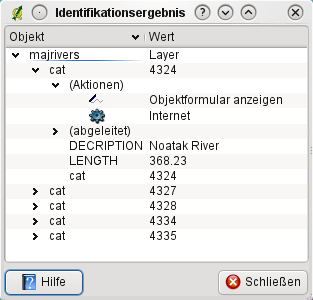
\includegraphics[clip=true, width=8cm]{action_identifyaction} 
\end{center}  
\end{figure}

Quando si clicca sull'azione, viene laciato Firefox all'URL
\url{http://www.google.com/search?q=Tustumena}. È anche possibile aggiungere
ulteriori campi all'azione, inserendo un ``+'' alla fine della stringa che
definisce l'azione, selezionando quindi un altro campo e cliccando sul
pulsante \button{Inserisci campo}. Nell'esempio seguito finora semplicemente non c'è alcun
altro campo sul quale avrebbe senso fare una ricerca.

È possibile definire più di un'azione per ogni layer, ognuna di esse verrà
mostrata nella finestra \dialog{Risultati individuati}. Si possono anche
eseguire azioni dalla tabella attributi cliccando con il tasto destro su una
riga selezionata e scegliendo dal menu contestuale l'azione desiderata.

Si possono immaginare molti tipi di azione. Ad esempio se un layer di punti
rappresenta le posizioni alle quali sono state scattate foto o alle quali
corrispondono immagini e il nome dei file di tali foto o immagini, è possibile
creare un'azione per lanciare un visualizzatore che mostri l'immagine. Le
azioni possono essere uate anche per lanciare report sul web per uno o più
campi della tabella attributo, definendole allo stesso modo definito
nell'esempio per la ricerca con Google.

\subsubsection{Scheda Attributi}\index{attributi}\label{label_attributes}
Nella scheda \tab{Attributi} è possibile modificare lo schema degli
attributi del layer selezionato. I pulsanti \button{Nuova colonna} ed
\button{Elimina colonna} vengono attivati quando il layer è in modalità
modifica, ovvero quando viene premuto il pulsante  \button{Alterna la modalità di modifica}. Al momento possono essere editate solo colonne appartenenti a layer
PostGIS, in quanto questa funzione non è ancora supportata dalla libreria OGR. 

\minisec{modifica widget}

Nella scheda \tab{Attributi} sono presenti anche le colonna
\texttt{modifica widget} e \texttt{valori}. Esse possono essere usate per
definire un valore o un campo di valori che possono essere aggiunti alla
specifica colonna della tabella attributi. 
Sono usati per produrre diversi "widgets" di modifica nella finestra degli
attributi. Questi "widgets" sono:

\begin{itemize}
\item modifica linea: un campo di modifica che consente di inserire un linea
di testo semplice (o esclusivamente numeri se l'attributo è di tipo numerico).
\item valori univoci: una lista di singoli valori da assegnare all'attributo
proveniente da elementi preesistenti viene prodotta e presentata in una combo
box per la selezione.
\item valori univoci (modificabile): una combinazione di `modifica linea' e
`valori univoci'. Il campo modifica consente di modificare i valori
preesistenti o di inserirne di nuovi.
\item valore mappa: una combobox nella quale è possibile scegliere da un
insieme di valori specificati nella colonna \texttt{valori} della scheda
\tab{Attributi}. I valori possibili sono delimitati da un punto e virgola (ad es.
\verb|high;medium;low|). È anche possibile preporre un'etichetta ad ogni
valore, la quale sarà delimitata dal segno dell'uguale (ad es.
\verb|high=1;medium=2;low=3|). L'etichetta è mostrata nella combobox al posto
del valore.
\item classificazione: if a unique value renderer is selected for the layer, the
values used for the classes are presented for selection in a combobox.
\item intervallo (modificabile): un campo di modifica che consente di
restringere i valori numerici entro un certo intervallo. L'intervallo viene
specificato inserendo i valori massimi e minimi delimitati da un punto e virgola (ad
es.\verb|0;360|) nella colonna \texttt{valori} della scheda \tab{Attributi}.
\item intervallo (cursore): un cursore scorrevole che consente la selezione di
un valore entro un predefinito intervallo e con una certo passo.
L'intervallo è definito da un valore minimo, massimo e dall'ampiezza del passo
(ad es. \verb|0;360;10|) nella colonna \texttt{valori} della scheda \tab{Attributi}.
\item nome file: la linea di editazione del "widget" presenta anche un
pulsante. Premendo il pulsante si può caricare un file usando la finestra di
dialogo per l'esplorazione delle risorse.
\end{itemize}

\subsection{Modifica}\index{modifica}

QGIS fornisce capacità basilari di editazione delle geometrie vettoriali.
Prima di procedere si evidenzia che a questo stadio il supporto per la modifica
è ancora preliminare.
Prima di eseguire una qualunque operazione di modifica, quindi, fare sempre una
copia di backup dei dati che si intendono modificare. 

\textbf{Nota} - la procedura per la modifica di layer GRASS è differente, si
veda la Sezione \ref{grass_digitising} per dettagli.

\begin{Tip}[ht]\caption{\textsc{Concurrent Edits}}
\qgistip{This version of QGIS does not track if somebody else is editing a
feature at the same time as you. The last person to save their edits wins.
}
\end{Tip}

\subsubsection{Settare la tolleranza dello snapping e il raggio di ricerca
degli elementi}

Prima di editare vertici, è molto importante sia impostare il livello di snapping
che il valore del raggio di ricerca che ci consentano una modifica ottimale delle
geometrie del layer vettoriale. 

\minisec{Tolleranza sullo snapping}

La tolleranza sullo snapping è la distanza entro la quale QGIS
\usertext{cerca} il più vicino vertice e/o segmento al quale si cerca di
agganciarsi quando si crea un nuovo vertice o si sposta un vertice esistente.
Se non si è entro la tolleranza di snapping, QGIS lascerà il vertice creato o
spostato nella posizione in cui si rilascia il pulsante del mouse invece di
agganciarlo ad un vertice e/o segmento esistente. 

\begin{enumerate}
\item Una prima impostazione della tolleranza sullo snapping può essere
impostata a livello dell'intero progetto scegliendo la voce di menu \mainmenuopt{Impostazioni} > \dropmenuopttwo{mActionOptions}{Opzioni}
Alla scheda \tab{Digitalizzazione} è possibile impostare la modalità di
snap predefinita tra snap al vertice, al segmento o entrambe. Si può anche
definire una tolleranza sullo snap e un raggio di ricerca per la modifica di
un vertice, in unità del layer. Nel set di dati Alaska, le unità sono in piedi
(feet). L'impostazione ottimale può variare, ma in genere 300 piedi può essere
una impostazione ragionevole per lavorare alla scala 1:10.000.
\item È anche possibile impostare una tolleranza sullo snapping basata sul
singolo layer scegliendo la voce di menu \mainmenuopt{Impostazioni} >
\dropmenuopttwo{mActionOptions}{Proprietà progetto\dots}. Nella scheda
\tab{Generale}, alla sezione \classname{Digitalizzazione} si può cliccare sul
pulsante \button{Opzioni di snap\dots} per abilitare e impostare la tolleranza
per ogni singolo layer del progetto (si veda la Figura~\ref{fig:snappingoptions}).
\end{enumerate}

\begin{figure}[H]
   \begin{center}
   \caption{Modifica delle opzioni di snapping per singoli layer \nixcaption}\label{fig:snappingoptions}\smallskip
   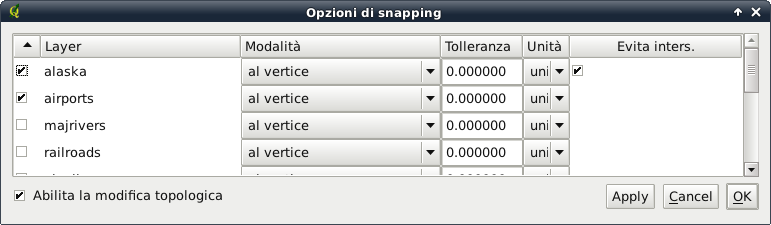
\includegraphics[clip=true, width=14cm]{editProjectSnapping} 
\end{center}  
\end{figure}

\minisec{Raggio di ricerca}

Il raggio di ricerca è la distanza che QGIS usa per \usertext{cercare} il più
vicino vertice che si sta cercando di spostare quando si clicca nella mappa.
Se non si è entro il raggio di ricerca, QGIS e mostrerà un avvertimento in
merito in una finestra pop-up.
La tolleranza sullo snap e il raggio di ricerca sono impostati in unità di
mappa e potrebbe essere necessario fare diversi tentativi per trovare
l'impostazione migliore. Se si specifica una tolleranza troppo alta, QGIS
potrebbe agganciare il vertice sbagliato, specialmente se si ha a che fare con
molti vertici vicini all'area in cui si sta effettuando la modifica.
Impostando invece un raggio di ricerca troppo piccolo impedirà invece a QGIS
di trovare alcuna geometria da spostare.

Il raggio di ricerca per la modifica di vertici può essere definita in unità
del layer dalla scheda \tab{Digitalizzazione} sotto il menu
\mainmenuopt{Impostazioni} -> \dropmenuopttwo{mActionOptions}{Opzioni}, sotto lo
stesso percorso dal quale è possibile impostare la tolleranza sullo snapping a
livello di progetto.

\subsubsection{Modifiche topologiche}

Oltre alle opzioni di snap a livello di singolo layer la scheda
\tab{Generale} sotto la voce di menu \mainmenuopt{Impostazioni} ->
\dropmenuopttwo{mActionOptions}{Proprietà progetto\dots} fornisce anche alcune
funzionalità per la topologia. 
Alla voce Digitalizzazione è possibile selezionare l'opzione \checkbox{Abilita
la modifica topologica} e/o attivare l'opzione \checkbox{Vieta le intersezioni
per i nuovi poligoni}.

\minisec{Abilitare la modifica topologica}

L'opzione \checkbox{Abilita la modifica topologica} serve a mantenere limiti
comuni tra poligoni adiacenti durante l'editazione. QGIS "individua" un limite
condiviso in un insieme di poligoni e tutto ciò che si deve fare è spostare il
vertice una volta sola, QGIS si occuperà di aggiornare anche il limite del
poligono adiacente.

\minisec{Impedire le intersezioni per i nuovi poligoni}

La seconda opzione \checkbox{VIeta intersezioni per i nuovi poligoni}
impedisce la sovrapposizione di poligoni adiacenti, rendendone più spedita la
digitalizzazione. Se si ha già un poligono, è possibile con questa opzione
abilitata digitalizzare il secondo in modo che entrambi si intersechino, QGIS
taglierà automaticamente il secondo sul limite comune con il vantaggio che
l'utente non deve digitalizzare tutti i vertici coincidenti.

\subsubsection{Modifica di un layer esistente}
\index{layer vettoriali!modifica}
\index{modifica!layer esistente}
\label{sec:edit_existing_layer}

Di default i layer sono caricati in QGIS in modalità solo lettura al fine di
evitare modifiche involontarie.
Comunque è sempre possibile modificare i layer se è consentito dalla
libreria (ovvero se ad es. OGR supporta lo specifico formato in
lettura/scrittura) e se il dato medesimo è anche scrivibile (ovvero i file
non sono in modalità sola lettura).

Le funzioni di modifica di layer sono più versatili quando sono applicate a
dati immagazzinati in database PostgreSQL/PostGIS. 

\begin{Tip}[ht]\caption{\textsc{Integrità del dato}}
\qgistip{È buona norma fare un back-up del dato originale prima di procedere
alla modifica. Per quando siano stati fatti molti sforzi da parte dei
programmatori di QGIS per preservare l'integrità del dato, non vi è alcuna
garanzia che ciò avvenga.
}
\end{Tip}

\begin{Tip}[ht]\caption{\textsc{Modifica di attributi}}
\qgistip{Attualmente solo ai layer PostGIS possono essere aggiunte o
eliminate colonne attributi da questa finestra. Nelle versioni di QGIS future
saranno supportate altre fonti di dati, in quanto questa caratteristica è
stata recentemente introdotta nelle librerie GDAL/OGR > 1.6.0
}
\end{Tip}



\begin{Tip}[ht]\caption{\textsc{Salvataggio ad intervalli regolari}}
\qgistip{Si ricordi di cambiare lo stato dello strumento
\toolbtntwo{mActionToggleEditing}{Abilita/disabilita modifica} ad intervalli
regolari, in modo da consentire il salvataggio delle modifiche recenti e per
verificare che le stesse siano accettate dalla sorgente di dati.
}
\end{Tip}

\begin{Tip}[ht]\caption{\textsc{Modifiche concorrenti}}
\qgistip{Questa versione di QGIS non effettua alcuna verifica sulla
possibilità che più utenti stiano effettuando contemporaneamente modifiche
sullo stesso layer, è quindi l'ultimo utente che effettua il salvataggio ad
apportare le modifiche definitive.
}
\end{Tip}

\begin{Tip}[ht]\caption{\textsc{Ingrandire prima della modifica}}
\qgistip{Prima di modificare un layer, bisognerebbe effettuare un
ingrandimento all'area di interesse, in modo da evitare che in modalità
modifica tutti i marker dei vertici visibili vengano resi a video per l'intero
layer.
}
\end{Tip}

\begin{Tip}[ht]\caption{\textsc{Marker dei vertici}}
\qgistip{
La versione di QGIS attuale supporta due tipi di marker per i vertici (in
modalità modifica): un
cerchio semitrasparente o una croce. Per cambiare lo stile del marker,
scegliere la voce \dropmenuopttwo{mActionOptions}{Opzioni} dal menu
\mainmenuopt{Impostazioni}, cliccare sulla scheda \tab{Digitalizzazione} e
selezionare la voce appropriata.
}
\end{Tip}

Ogni sessione di modifica può essere inizializzata dall'opzione
\dropmenuopttwo{mActionToggleEditing}{Attiva/disattiva modifica}, che può
essere attivata e disattivata cliccando con il tasto destro sul nome del layer nella legenda e scegliendo dal menu contestuale \index{attiva/disattiva modifica} oppure
dalla barra strumenti cliccando sul pulsante \index{attiva/disattiva modifica}
\toolbtntwo{mActionToggleEditing}{Attiva/disattiva
modifica}.\index{modifica!icone} Quando il layer è in modalità modifica, i
vertici verranno contrassegnati dai markers impostati (croci o cerchi
semitrasparenti) e ulteriori pulsanti verranno resi disponibili nella barra
degli strumenti di modifica.

\minisec{Zoom con la rotella del mouse}

Mentre si digitalizza è possibile usare la rotella del mouse per ingrandire e
ridurre la mappa, posizionando il cursore nell'area di mappa e girando la
rotellina verso di sé per ridurre e verso lo schermo per ingrandire. La
posizione del puntatore del mouse determinerà centro dell'area da
ingrandire. È possibile personalizzare il comportamento della rotella del
mouse nella scheda \tab{Strumenti mappa} alla voce di munù \mainmenuopt{Impostazioni} 
>\dropmenuopt{Opzioni}.

\minisec{Spostare la vista mappa con i tasti freccia}

È possibile spostare la vista mappa mentre si digitalizza aiutandosi con i
tasti freccia, posizionando il puntatore del mouse nella vista e cliccando
sulla freccia destra per spostarsi verso est, sinistra per spostarsi verso ovest,
su per spostarsi verso nord e giù per andare verso sud.

È anche possibile tenere premuta la barra spaziatrice mentre si sposta il
mouse per spostare la vista mappa e usare i tasti PgUp e PgDown per aumentare
o ridurre l'ingrandimento senza interrompere la sessione di digitalizzazione.

Sono disponibili le seguenti funzioni di modifica:

\begin{itemize}
\item Aggiunta elementi: \toolbtntwo{mActionCapturePoint}{Inserisci punti},
  \toolbtntwo{mActionCaptureLine}{Inserisci linee} and
  \toolbtntwo{mActionCapturePolygon}{Inserisci poligoni}
\item \toolbtntwo{mActionAddRing}{Inserisci anello}
\item \toolbtntwo{mActionAddIsland}{Inserisci isola}
\item \toolbtntwo{mActionSplitFeatures}{Dividi geometria}
\item \toolbtntwo{mActionMoveFeature}{Sposta geometria}
\item \toolbtntwo{mActionMoveVertex}{Sposta vertice}
\item \toolbtntwo{mActionAddVertex}{Aggiungi vertice}
\item \toolbtntwo{mActionDeleteVertex}{Elimina vertice}
\item \toolbtntwo{mActionDeleteSelected}{Elimina selezione}
\item \toolbtntwo{mActionEditCut}{Taglia geometrie}
\item \toolbtntwo{mActionEditCopy}{Copia geometrie}
\item \toolbtntwo{mActionEditPaste}{Incolla geometrie}
\end{itemize}

\minisec{Aggiungere elementi}
\index{layer vettoriali!aggiungere!elemento}

Prima di iniziare ad aggiungere elementi ad un layer, usare gli strumenti
\toolbtntwo{mActionPan}{Sposta mappa} \toolbtntwo{mActionZoomIn}{Ingrandisci} \toolbtntwo{mActionZoomOut}{Rimpicciolisci}
per visualizzare l'area di mappa nella quale si desidera apporre modifiche.

A questo punto si possono usare gli strumenti \toolbtntwo{mActionCapturePoint}{Inserisci punti},
\toolbtntwo{mActionCaptureLine}{Inserisci linee} o
\toolbtntwo{mActionCapturePolygon}{Inserisci poligoni} per porre il puntatore
di QGIS in modalità digitalizzazione.

Per ogni elemento, bisogna dapprima digitalizzarne la geometria e
successivamente inserirne gli attributi.

Per digitalizzare la geometria, cliccare con il tasto sinistro sull'area di
mappa per creare il primo punto del nuovo elemento.

Per linee e poligoni, continuare a cliccare con il tasto sinistro per ogni
ulteriore vertice che si desidera inserire. Quando è terminato l'inserimento
dei vertici o dei punti, cliccare con il tasto destro in qualunque punto della
mappa per confermare di aver terminato l'inserimento della geometria
dell'elemento.

Apparirà quindi la finestra degli attributi che consentirà di inserire le
informazioni per l'elemento appena creato.
La Figura \ref{fig:vector_digitising} mostra l'inserimento degli attributi per
un fiume fittizio creato in Alaska.

\begin{figure}[ht]
   \begin{center}
   \caption{Finestra di inserimento degli attributi per un elemento di nuova
   digitalizzazione \nixcaption}\label{fig:vector_digitising}\smallskip
   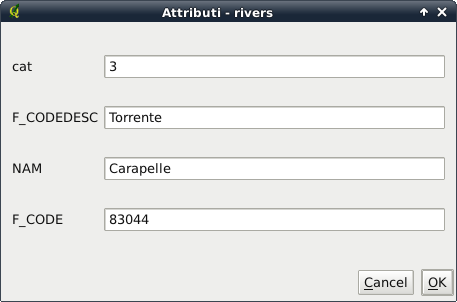
\includegraphics[clip=true, width=8cm]{editDigitizing}
\end{center}  
\end{figure}

\begin{Tip}[ht]\caption{\textsc{Tipologie di attributo}}
\qgistip{
Almeno per gli shapefile la modifica del tipo di attributo è validata durante
l'inserimento. A causa di ciò, non è ovviamente possibile inserire un numero
in una colonna testuale quando compare la finestra \dialog{Inserire i valori
dell'attributo} o viceversa. Se ciò fosse necessario, si dovrebbero modificare
gli attributi in un secondo momento per mezzo della finestra \dialog{Tabella
attributo}.
}
\end{Tip}

\minisec{Spostare elementi}
\index{layer vettoriali!spostare!elemento}

Si possono spostare elementi scegliendo dalla barra lo strumento
\toolbtntwo{mActionMoveFeature}{Sposta geometria}.

\minisec{Dividere elementi}
\index{layer vettoriali!dividere!elemento}

Si possono dividere elementi scegliendo dalla barra lo strumento \toolbtntwo{mActionSplitFeatures}{Dividi geometria}.

\minisec{Modificare i vertici di un elemento}
\index{layer vettoriali!modificare!vertice}

Sia per i layer PostgreSQL/PostGIS che per gli shapefile, i vertici di un
elemento possono essere modificati. 

I vertici possono essere modificati direttamente senza che si debba
selezionare l'elemento del quale si voglia modificare la geometria.
In alcuni casi, più elementi possono condividere dei vertici, in questi casi
valgono le seguenti regole quando si clicca con il mouse vicino ad un elemento
del layer:

\begin{itemize}
\item \textbf{Linee}    - La linea più vicina al cursore è scelta come
                          elemento da modificare.
                          Di conseguenza (per spostare e cancellare vertici)
                          viene selezionato per la modifica il vertice
                          più vicino su quella linea.

\item \textbf{Polygoni} - Se il mouse è all'interno di un poligono, esso è
                          l'elemento da modificare; altrimenti viene usato il più vicino
			  poligono.
                          Di conseguenza (per spostare e cancellare vertici)
                          viene selezionato per la modifica il vertice più
			  vicino su quel poligono.
\end{itemize}

Ricordarsi di impostare l'opzione sotto
\mainmenuopt{Impostazioni}>\dropmenuopttwo{mActionOptions}{Opzioni}>\tab{Digitalizzazione}
alla casella \selectnumber{Raggio di ricerca per la modifica di un vertice in unità layer}{10}
ad un valore superiore a zero, altrimenti QGIS non sarà in grado di
determinare quale elemento deve essere modificato.


\minisec{Aggiungere vertici ad un elemento}
\index{layer vettoriali!aggiungere!vertice}

Si possono aggiungere ulteriori vertici ad un elemento del layer scegliendo
dalla barra lo strumento \toolbtntwo{mActionAddVertex}{Aggiungi vertice}.

Si noti che è privo di senso aggiungere ulteriori vertici ad un elemento
puntuale!

In questa versione di QGIS i vertici possono essere aggiunti sono ad un
segmento di elementi lineari \textit{esistenti}. Se si desidera estendere una
linea oltre le sue estremità, è necessario spostare dapprima il vertice finale
e quindi aggiungere un nuovo vertice nel punto in cui questo si trovava.

\minisec{Spostare i vertici di un elemento}
\index{layer vettoriali!spostare!vertice}

Si possono spostare vertici scegliendo dalla barra lo strumento \toolbtntwo{mActionMoveVertex}{Sposta vertice}.

\minisec{Cancellare vertici di un elemento}
\index{layer vettoriali!cancellare!vertice}

Si possono cancellare vertici scegliendo dalla barra lo strumento \toolbtntwo{mActionDeleteVertex}{Elimina vertice}.

Si noti che è privo di senso cancellare un vertice da un elemento puntuale,
poiché questo equivarrebbe a cancellare l'elemento!

Similmente una linea costituita da un solo vertice o un poligono costituito da
due vertici non hanno molto senso e potrebbero avere comportamenti imprevisti
nell'uso di altre funzioni di QGIS (ad es. con gli strumenti di analisi) e di
conseguenza bisogna evitare modifiche che portino a creare tali geometrie.

\textbf{Attenzione:} Un vertice è contrassegnato per l'eliminazione non appena
si clicca con il mouse vicino ad un elemento selezionabile. Per annullare,
sarà necessario disabilitare la modalità di modifica senza salvare i
cambiamenti. (Ovviamente questo comporterà anche la perdita delle altre
modifiche non salvate.)

\minisec{Inserisci anello (buco)}
\index{layer vettoriali!inserire!anello}

So possono digitalizzare nuovi poligoni all'interno di poligoni esistenti al fine
di creare un buco all'interno di questi ultimi scegliendo dalla barra lo
strumento \toolbtntwo{mActionAddRing}{Inserisci anello}.
In questo modo solo l'area compresa tra i margini del poligono interno e di
quello esterno verrà evidenziata come un poligono ad anello. 

\minisec{Inserisci isola, ovvero creazione/modifica di un multipoligono}
\index{layer vettoriali!inserire!isola}

Si possono creare e modificare multipoligoni (insieme di elementi poligonali
geometricamente indipendenti ovvero non condividenti alcun vertice o limite
visti come entità unica quando si seleziona anche uno solo dei singoli
elementi) aggiungendo ulteriori "isole" ad
un singolo poligono o ad un multipoligono esistenti scegliendo dalla barra lo
strumento \toolbtntwo{mActionAddIsland}{Inserirsci isola}. La nuova "isola"
del multipoligono deve essere esterna al poligono che si intende rendere
multipoligono o agli elementi già facenti parte di un multipoligono esistente
che si intende modificare. 

\minisec{Tagliare, copiare ed incollare elementi}
\index{layer vettoriali!tagliare!elemento}
\index{layer vettoriali!copiare!elemento}
\index{layer vettoriali!incollare!elemento}
\index{modifica!tagliare elementi}
\index{modifica!copiare elementi}
\index{modifica!incollare elementi}

Gli elementi selezionati possono essere tagliati, copiati ed incollati
tra layer dello stesso progetto di QGIS a patto che anche nel layer di destinazione
sia stata abilitata la modalità di modifica tramite l'opzione 
\toolbtntwo{mActionToggleEditing}{Attiva/disattiva modifica}.

Gli elementi possono essere anche incollati in applicazioni esterne come testi: gli elementi verrano rappresentati nel formato CSV con le informazioni della geometria espresse nel formato testo OGC Well-Known Text (WKT).

Tuttavia in questa versione di QGIS elementi di testo formattato creati con
applicazioni esterne non possono essere incollate in un layer dentro QGIS.

Le funzioni di copia/incolla possono essere utili quando si vogliano modificare più layer copiando le modifiche effettuate in uno di questi negli
altri. Supponendo ad esempio di voler lavorare su un layer contenente un paio
di laghi, diventa molto più agevole creare un nuovo layer vuoto nel quale
incollare gli elementi dei quali necessitiamo invece di lavorare sul layer \filename{big\_lakes} contenente 5000 elementi. 

Dovremo quindi effettuare le seguenti operazioni:

\begin{enumerate}
\item Caricare il layer dal quale vogliamo copiare gli elementi (layer
sorgente)
\item Caricare o creare il layer nel quale vogliamo incollare gli elementi
copiati(layer di destinazione) 
\item Impostare entrambi i layer in modalità modifica 
\item Rendere attivo il layer sorgente cliccando sul relativo nome nella
legenda 
\item Attivare lo strumento \toolbtntwo{mActionSelect}{Seleziona geometrie}
per selezionare gli elementi dal layer sorgente
\item Cliccare sullo strumento \toolbtntwo{mActionEditCopy}{Copia geometrie}
\item Rendere attivo il layer di destinazione cliccando sul relativo nome
nella legenda
\item Attivare lo strumento \toolbtntwo{mActionEditPaste}{Incolla geometrie} 
\item Terminare le modifiche e salvare
\end{enumerate}

Se il layer sorgente e quello di destinazione hanno un diverso schema (nomi e
tipi dei campi) della
tabella attributi QGIS popola, (se presenti) i campi comuni e ignora il resto.
Se non è importante che vengano copiati anche gli attributi nel layer di
destinazione, si può non prestare attenzione a come viene definito lo schema
della tabella attributi, altrimenti è necessario definirlo in modo che quello
del layer sorgente e di destinazione combacino.

\begin{Tip}[ht]\caption{\textsc{Congruenza degli elementi incollati}}
\qgistip{Se il layer sorgente e quello di destinazione usano lo stesso sistema
di proiezione, gli elementi incollati saranno assolutamente identici a quelli
del layer di origine. Nel caso in cui invece la proiezione del layer di
destinazione sia differente QGIS non garantisce che la geometria sia identica
a causa del pur ridotto errore di arrotondamento introdotto nel passaggio da
un sistema di proiezione all'altro.
}
\end{Tip}

\minisec{Cancellare elementi selezionati}
\index{layer vettoriali!cancellare!elemento}

Se si vuole eliminare un intero poligono, è possibile farlo selezionando
dapprima l'elemento che intendiamo cancellare con lo strumento
\toolbtntwo{mActionSelect}{Seleziona geometrie}. È possibile anche selezionare
contemporaneamente più poligoni da cancellare in una volta sola. Una volta
definita la selezione, usare lo strumento
\toolbtntwo{mActionDeleteSelected}{Elimina selezione} per cancellare la
selezione. Non è possibile annullare l'eliminazione, tuttavia è sempre
possibile annullare l'eliminazione (ma anche altre eventuali modifiche
effettuate dall'ultimo salvataggio!) terminando la modalità di modifica senza
salvare le modifiche.

Anche lo strumento \toolbtntwo{mActionEditCut}{Taglia geometrie} può essere
usato per eliminare elementi, che vengono in questo caso spostati un un
"blocco appunti spaziale". In questo modo è però possibile annullare
l'operazione incollando nuovamente gli elementi tagliati con lo strumento
\toolbtntwo{mActionEditPaste}{Incolla geometrie} fornendo in ultima
analisi almeno un livello di annullamento.

Tutti gli strumenti taglia, copia e incolla lavorano sugli elementi
attualmente selezionati, consentendo quindi di lavorare su più di un elemento
alla volta.

\begin{Tip}[ht]\caption{\textsc{Supporto alla cancellazione di elementi}}
\qgistip{Quando si modificano shapefile, la cancellazione di elementi
funziona solo se QGIS è compilato contro una versione di GDAL pari a 1.3.2 o
superiore, come accade per le versioni compilate per OS X and Windows
disponibili sul sito.
}
\end{Tip}

\minisec{Modalità di snap}
\index{modifica!snap}
QGIS consente di agganciare i vertici digitalizzati ad altri vertici dello
stesso layer. Per impostare la tolleranza di aggancio, andare alla voce di
menu \mainmenuopt{Impostazioni}>\dropmenuopttwo{mActionOptions}{Opzioni}->\tab{Digitalizzazione}.
Si noti che la tolleranza di aggancio è in unità di mappa.

\minisec{Salvare i layer modificati}
\index{modifica!salvare modifiche}

Quando un layer è in modalità modifica, tutti i cambiamenti rimangono nella
memoria di QGIS e quindi non sono immediatamente applicati e salvati nei dati
su disco. Quando viene disabilitata la modalità di modifica (o si termina la
sessione di QGIS mentre questa non è stata finalizzata), 
viene chiesto se si desidera salvare o scartare le modifiche.

Se le modifiche non possono essere salvate (ad es. perché il disco di
destinazione è pieno o gli attributi contengono valori esterni agli estremi
ammissibili), lo stato della memoria di QGIS è preservato, consentendo dunque
di correggere gli errori e riprovare il salvataggio.

\subsubsection{Creare un nuovo layer}\label{sec:create shape}\index{modifica!creare un nuovo layer}

Per creare un nuovo layer da modificare, scegliere l'opzione
\toolbtntwo{mActionNewVectorLayer}{Nuovo layer vettoriale} dal menu \mainmenuopt{Layer}. 
Verrà quindi aperta la finestra \dialog{Nuovo layer vettoriale} come mostrato
in Figure \ref{fig:newvectorlayer}. Scegliere qui il tipo di geometria che si
intende inserire nel layer (punto, linea o poligono).

\begin{figure}[ht]
   \begin{center}
   \caption{Finestra di creazione di un nuovo layer vettoriale \nixcaption}\label{fig:newvectorlayer}\smallskip
   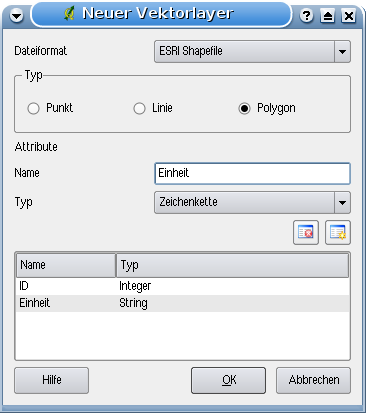
\includegraphics[clip=true, width=10cm]{editNewVector}
\end{center} 
\end{figure}

Si noti che QGIS non supporta la creazione di elementi 2.5D (ad es. elementi
con coordinate XYZ) o il conteggio degli elementi. Ad oggi inoltre possono
essere creati solo shapefile. Il supporto per la creazione di layer OGR o
PostgreSQL sarà inserito in future versioni di QGIS. 

La creazione di layer di GRASS è supportata dal plugin GRASS. Si faccia
riferimento alla Sezione \ref{sec:creating_new_grass_vectors} per ulteriori
informazioni sulla creazione di layer vettoriali GRASS.

Per completare la creazione del nuovo layer, si definisca lo schema degli
attributi specificando il nome e tipo della colonna da inserire nella tabella
e cliccando sul pulsante \button{Aggiungi attributo}. Sono supportati solo
attributi di tipo \selectstring{Tipo}{real}, \selectstring{Tipo}{Intero}, and
\selectstring{Tipo}{Stringa}. Una volta definito lo schema, cliccare su
\button{OK} e assegnare un nome allo shapefile.
QGIS aggiungerà automaticamente l'estensione \filename{.shp} al nome indicato.
Una volta creato il layer, esso sarà aggiunto alla mappa e potrà essere
modificato nello stesso modo descritto alla precedente Sezione \ref{sec:edit_existing_layer}. 

\subsection{Generatore di query (query builder)}\label{sec:query_builder}
\index{generatore di query}

Il generatore di query consente di definire (tramite il linguaggio Structured
Query Language, SQL) un sottoinsieme di una tabella e mostrarlo come layer in
QGIS. Può essere usato pper tutti i formati OGR, i file di GRASS ed i layer
di PostGIS. 
Per esemio, se si ha il file \filename{towns} che contiene un campo
\usertext{population} nella tabella attributi indicante il numero di residenti
è possibile selezionare solo le città più grandi inserendo l'espressione
\usertext{population > 100000} nella casella SQL del costruttore di query. La
Figura \ref{fig:query_builder} mostra un esempio per il costruttore di query
popolato con dati provenienti da layer PostGIS immagazzinati nel database PostgreSQL. 

\begin{figure}[ht]
  \begin{center}
    \caption{La finestra del costruttore di query \nixcaption}\label{fig:query_builder}\smallskip
    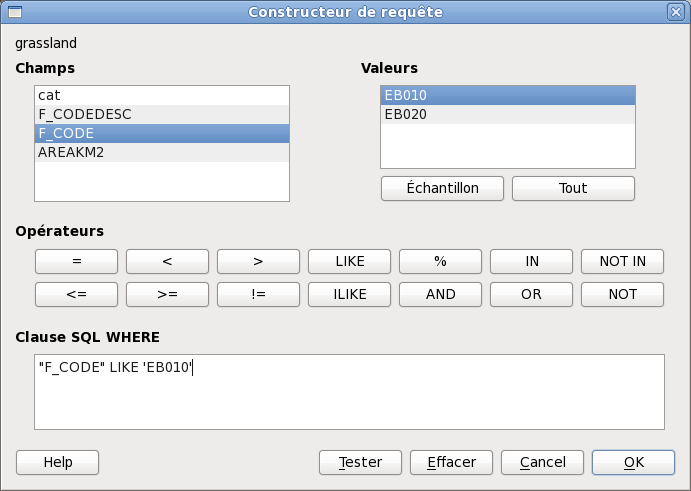
\includegraphics[clip=true, width=11.5cm]{queryBuilder}
  \end{center}  
\end{figure}

La finestra del costruttore di query\index{generatore di query} elenca i campi del
database nella casella sulla sinistra. Un campione dei dati selezionabili con
l'espressione impostata è visibile cliccando sul pulsante \button{Campione} \index{generatore di query!generare un campione dei dati}. In questo modo vengono richiamati i primi 25
valori distinti dai campi del database. Per avere una lista completa di tutti
i valori di un campo, cliccare sul pulsante \button{All} \index{generatore di query!ottenere tutti
i valori}. Per aggiungere un campo o un valore selezionato alla query, fare
doppio-click su di esso\index{generatore di query!aggiungere campi}. È possibile usare
i vari pulsanti per costruire le interrogazioni oppure digitare direttamente
il testo dell'interrogazione nella casella SQL.

Per provare una query cliccare sul pulsante \button{Prova}
\index{generatore di query!provare query}. Se l'espressione è correta, verrà
restituito un conteggio dei record che verranno inclusi nella selezione.
Quando l'espressione dell'interrogazione è soddisfacente, cliccare sul
pulsante \button{OK}. Nella casella SQL verrà mostrato il testo della richiesta.

\begin{Tip}\caption{\textsc{Cambiare la definizione di un layer}}\index{generatore di query!cambiare la definizione di un layer}
\qgistip{Si può cambiare la definizione SQL di un layer caricato da PostGIS anche dopo che questo è stato caricato, aprendo la finestra \dialog{Proprietà del vettoriale}
facendo doppio click sul nome del layer nella legenda e cliccando sul pulsante
\button{Query Builder} nella scheda \tab{Generale}. Si veda la Sezione
\ref{sec:vectorprops} per ulteriori informazioni.}
\end{Tip}

\subsection{Selezione mediante interrogazione}\label{sec:select_by_query}
\index{PostgreSQL!generatore di query}
\index{PostGIS!generatore di query}
\index{generatore di query!PostgreSQL}
\index{generatore di query!PostGIS}

Con QGIS è possibile selezionare elementi per mezzo di un'interfaccia simile a
quella del generatore di query usata in \ref{sec:query_builder}.
Nella sezione precedente il generatore di query è stato usato unicamente per
mostrare gli elementi di un layer che soddisfacevano i filtri imposti in un
"layer virtuale" sottoinsieme di quello originale. Lo scopo della selezione
mediante interrogazione è invece quello di evidenziare gli elementi di un
layer caricato che soddisfano particolare criteri.
La selezione con query può essere usata con tutte le sorgenti di dati
vettoriali supportate.

Per effettuare una selezione mediante interrogazione su un layer caricato,
cliccare sul pulsante \toolbtntwo{mActionOpenTable}{Apri tabella attributi}
e cliccare nella finestra sul pulsante \button{Advanzate...} in basso a
destra. In questo modo viene avviato il generatore di query che
consente di definire un sottoinsieme degli elementi e mostrarli come descritto
alla Sezione \ref{sec:query_builder}.


\index{layer vettoriali|)}
